% =====================================================================
%  Paper teórico — versión standalone para envío a revista
%  Un microfundamento de organización industrial para la fragilidad
%  bancaria sistémica y el riesgo soberano
%
%  Reutiliza el cuerpo del Capítulo 3 de la tesis (../../tesis/paper1_oi.tex)
%  + el Anexo A matemático (../../tesis/anexoA_matematico.tex) como apéndice.
%  Revistas objetivo (español): El Trimestre Económico, Estudios de Economía
%  (U. de Chile), Revista de Análisis Económico (ILADES).
% =====================================================================
\documentclass[12pt,letterpaper]{article}
\usepackage[spanish,es-tabla]{babel}
\usepackage[utf8]{inputenc}
\usepackage[T1]{fontenc}
\usepackage{amsmath,amssymb,amsthm}
\usepackage{booktabs}
\usepackage{array}
\usepackage{graphicx}
\usepackage{mdframed}
\usepackage{setspace}
\usepackage[margin=1in]{geometry}
\usepackage[hidelinks]{hyperref}
\usepackage{natbib}
\bibliographystyle{apalike}

\graphicspath{{figuras/}}
\setlength{\emergencystretch}{3em}
\onehalfspacing

\newcommand{\JLoss}{\mathrm{JLoss}}
\newcommand{\Spread}{\mathrm{spread}}
\newcommand{\GaR}{\mathrm{GaR}}
\newcommand{\PD}{\mathrm{PD}}
\newcommand{\ES}{\mathrm{ES}}
\newcommand{\HHI}{\mathrm{HHI}}
\newcommand{\Var}{\mathrm{Var}}
\newcommand{\dd}{\,\mathrm{d}}
% macros que la tesis hereda de umemoria.cls
\newcommand{\E}{\mathbb{E}}
\newcommand{\1}{\mathbf{1}}
\providecommand{\R}{\mathbb{R}}
\providecommand{\N}{\mathbb{N}}
\let\epsilon\varepsilon

\theoremstyle{plain}
\newtheorem{proposition}{Proposición}
\newtheorem{lemma}{Lema}
\theoremstyle{definition}
\newtheorem{definition}{Definición}
\newtheorem{assumption}{Supuesto}
\newtheorem{remark}{Observación}

% Re-enunciado de una proposición en el anexo matemático (numeración vía \ref).
\newcommand{\restateprop}[2]{%
  \par\medskip\noindent\textbf{Proposición~\ref{#1}.}\enspace\begingroup\itshape #2\endgroup\par\medskip}

\let\chapter\section
\makeatletter
\newcommand{\definelabel}[2]{\expandafter\gdef\csname r@#1\endcsname{{#2}{}{}{}{}}}
\makeatother
\definelabel{chap:paper2}{el trabajo empírico complementario}
\definelabel{chap:discusion}{la discusión general de la tesis}

\title{Estructura de mercado bancario, fragilidad sistémica y riesgo soberano:\\
un microfundamento de organización industrial}
\author{Mauricio Valenzuela Corvalán\\[2pt]
\small Magíster en Economía Aplicada, Universidad de Chile}
\date{\today}

\begin{document}
\maketitle

\begin{abstract}
\noindent
Este trabajo desarrolla un modelo formal en el que la \textit{estructura de mercado
bancario} es el parámetro profundo que gobierna la cadena que va desde la fragilidad
sistémica hasta el riesgo soberano. En un mercado de crédito con competencia à la
Cournot, responsabilidad limitada y seguro de depósitos, la intensidad de competencia
opera sobre el riesgo por dos canales de signo opuesto —efecto margen y efecto
\textit{risk-shifting}—, generando una relación en U con la probabilidad de quiebra
individual. El aporte central es distinguir el riesgo \emph{individual} del riesgo de
\emph{cola conjunta} del sistema ($\JLoss$): al endogenizar la correlación de activos
como función de la estructura de mercado, el mínimo de $\JLoss$ se ubica en un mercado
más competido que el de mínima fragilidad individual, de modo que una política de
competencia calibrada solo sobre la salud individual de los bancos deja al sistema en
una configuración subóptimamente concentrada desde la óptica del riesgo sistémico y de
su costo fiscal contingente. El cierre macro-soberano genera una complementariedad
entre fragilidad y riesgo a la baja del crecimiento sobre el \textit{spread} soberano,
que constituye el análogo teórico exacto del término de interacción $\JLoss\times\GaR$
que la evidencia empírica documenta. El modelo se ilustra numéricamente, se valida
contra Monte Carlo y sobrevive a una estructura de competencia alternativa (Salop) y a
una revisión adversarial explícita.\\[4pt]
\noindent\textbf{Palabras clave:} competencia bancaria, riesgo sistémico,
\textit{Growth-at-Risk}, riesgo soberano, \textit{doom loop}.\quad
\textbf{JEL:} G21, G28, E44, H63, L13.
\end{abstract}

\chapter{Un microfundamento de organización industrial bancaria para la complementariedad fragilidad--crecimiento}
\label{chap:paper1}

\section*{Resumen del capítulo}
\addcontentsline{toc}{section}{Resumen del capítulo}

Este capítulo desarrolla un modelo teórico formal en el que la \textit{estructura de mercado bancario} es el parámetro profundo que gobierna la cadena que va desde la fragilidad sistémica hasta el riesgo soberano en economías emergentes. En un mercado de crédito con competencia à la Cournot, responsabilidad limitada y seguro de depósitos, la intensidad de competencia opera sobre el riesgo por dos canales de signo opuesto ---efecto margen (Keeley) y efecto \textit{risk-shifting} (Boyd--De Nicoló)---, generando una relación en U con la probabilidad de quiebra individual (Proposición~\ref{prop:U}, que anida a \citealp{MMR2010}). El aporte central es distinguir el riesgo \textit{individual} del riesgo de \textit{cola conjunta} del sistema ($\JLoss$): al endogenizar la correlación de activos como función de la estructura de mercado, la concentración no solo desplaza la probabilidad de incumplimiento sino que engrosa la cola conjunta, de modo que el mínimo de $\JLoss$ se ubica en un mercado más competido que el de mínima fragilidad individual (Proposición~\ref{prop:shift}), y el traspaso de la cola es creciente en la concentración (Proposición~\ref{prop:granular}). El cierre macro-soberano ---un canal de \textit{credit crunch} ($\JLoss\!\to\!\GaR$) y un bloque de límite fiscal ($\GaR,\JLoss\!\to\!\Spread$)--- produce una complementariedad: el efecto de la fragilidad sobre el spread se amplifica cuando el crecimiento ya está en la cola, y esa amplificación crece con la concentración (Proposición~\ref{prop:cross}). Todas las proposiciones se ilustran numéricamente, el método de cálculo de $\JLoss$ se valida contra Monte Carlo, y el diseño empírico se valida primero por Monte Carlo (recuperación de los signos predichos $\beta_3,\beta_4>0$ ---en la convención de riesgo de cola $D\equiv-\GaR$--- en el 100\% de $3000$ réplicas) y luego se contrasta con un único panel de trece economías emergentes, con la fragilidad bancaria construida desde Bloomberg y el spread soberano medido por el EMBI Global Diversified. El contraste arroja un resultado \textbf{asimétrico}: la complementariedad de primer orden ($\beta_3>0$ en la parametrización de nivel sobre $D=-\GaR$; equiv.\ $\theta<0$ con $\GaR$) tiene el signo y la forma predichos —el efecto de la fragilidad sobre el spread crece a medida que empeora el riesgo de cola, y un modelo de umbral lo corrobora— pero su significancia estadística es \textbf{condicional}: se sostiene sobre el núcleo de once economías emergentes de financiamiento externo ($\hat\beta_3=+0{,}47$, $p=0{,}023$) y se diluye al añadir economías con mercados de deuda local profundos, sin que la diferencia entre grupos alcance un contraste formal. La predicción distintiva del modelo, la amplificación por concentración ($\beta_4$), \textbf{no puede contrastarse con potencia}: con trece países el punto estimado de $\hat\beta_4$ no tiene signo estable entre proxies de concentración y su intervalo de confianza robusto (\textit{bootstrap} de bloques por país) cruza el cero holgadamente con todos ellos —incluida una serie de concentración trimestral construida de los mismos balances Bloomberg que $\JLoss$. Se reporta este resultado con franqueza, junto con la explicación —descartada ya la falta de variación temporal del proxy— de que la homogeneización de la métrica de fragilidad al usar una sola fuente comprime la dispersión transversal sobre la que se identifica la triple interacción, o de que el canal es genuinamente más débil que su calibración, y con la agenda de datos que permitiría distinguir entre ambas. El modelo sobrevive además a una estructura de competencia alternativa (Salop) y a una revisión adversarial explícita.

\vspace{6pt}
\noindent\textbf{Palabras clave:} estabilidad financiera, competencia bancaria, riesgo sistémico, Growth-at-Risk, riesgo soberano, \textit{doom loop}.\\
\noindent\textbf{Clasificación JEL:} G21, G28, E44, H63, L13.

\section{Introducción}\label{sec:intro}

La relación entre competencia bancaria y estabilidad financiera es uno de los debates más persistentes de las macrofinanzas, y la evidencia empírica es abiertamente contradictoria. Por un lado, la hipótesis de \textit{competencia-fragilidad} \citep{Keeley1990} sostiene que la competencia erosiona el valor de la franquicia (\textit{charter value}) y comprime los márgenes, reduciendo el colchón de los bancos e incentivando la toma de riesgo. Por otro, la hipótesis de \textit{competencia-estabilidad} \citep{BoydDeNicolo2005} sostiene que un mayor poder de mercado eleva las tasas de préstamo, induce a los proyectistas a seleccionar proyectos más riesgosos (\textit{risk-shifting}) y aumenta la probabilidad de incumplimiento de la cartera. \citet{MMR2010} reconcilian ambas fuerzas en un mismo equilibrio y muestran que la relación entre competencia y riesgo de quiebra individual es en \textit{U}.

Este trabajo parte de esa reconciliación pero desplaza el objeto de interés. Para la estabilidad financiera y el riesgo soberano lo relevante no es la fragilidad de un banco representativo, sino la \textit{cola conjunta de pérdidas} del sistema —la magnitud de las pérdidas cuando muchos bancos fallan simultáneamente—, que se denota $\JLoss$ y que se computa en el marco de \citet{Merton1974} y la aproximación de punto de silla. La distinción es sustantiva: la competencia reduce monótonamente el riesgo del \textit{proyectista}, pero afecta de forma no trivial la \textit{correlación} de exposiciones entre bancos. La tesis central de este capítulo es que la estructura de mercado es el parámetro profundo que gobierna toda la cadena
\begin{equation*}
n\ (\text{estructura}) \;\longrightarrow\; \JLoss \;\longrightarrow\; \GaR \;\longrightarrow\; \Spread,
\end{equation*}
donde $\GaR$ es el \textit{Growth-at-Risk} en el sentido de \citet{ABG2019} y $\Spread$ denota el spread soberano en abstracto —su contraparte empírica en el Capítulo~\ref{chap:paper2} es el índice EMBI Global Diversified de J.P.\ Morgan, con el CDS soberano a cinco años como serie de robustez.

\paragraph{Contribución.} El modelo se apoya en un resultado técnico preliminar —existencia y unicidad del equilibrio de Cournot (Proposición~\ref{prop:exist})— sobre el cual el trabajo construye cuatro resultados económicos. Primero, recupera la relación en U de la fragilidad individual como caso particular (Proposición~\ref{prop:U}). Segundo ---y es la contribución marginal frente a \citet{MMR2010}---, al endogenizar la correlación de activos $\rho(n)$, el modelo muestra que el mínimo de la fragilidad \textit{sistémica} $\JLoss$ se desplaza hacia mayor competencia respecto del mínimo de la fragilidad individual (Proposición~\ref{prop:shift}): una política de competencia calibrada solo sobre la salud individual de los bancos deja al sistema en una configuración subóptimamente concentrada desde la óptica del riesgo de cola. Tercero, el traspaso de la cola sistémica es creciente en la concentración por un canal de granularidad (Proposición~\ref{prop:granular}). Cuarto, el cierre macro-soberano genera una complementariedad entre fragilidad y riesgo a la baja sobre el spread soberano, amplificada por la concentración (Proposición~\ref{prop:cross}), que constituye el análogo teórico exacto del término de interacción $\JLoss\times D$ (con $D\equiv-\GaR$) y su heterogeneidad por concentración que la literatura estima empíricamente.

\paragraph{Literatura relacionada.} El trabajo integra tres literaturas. La de \textit{organización industrial bancaria y estabilidad} \citep{Keeley1990,AllenGale2004,BoydDeNicolo2005,MMR2010,Vives2016}; la de \textit{riesgo sistémico} y medidas de pérdida conjunta \citep{Merton1974,Vasicek2002,Gordy2003,AcharyaEtAl2017,AdrianBrunnermeier2016}; y la de \textit{riesgos a la baja y nexo soberano-bancario} \citep{ABG2019,AcharyaDrechslerSchnabl2014,FarhiTirole2018,GhoshEtAl2013}. Ninguna de las tres, tomada por separado, deriva un objeto de fragilidad de \textit{cola conjunta} como función de la estructura de mercado bancario: la literatura de organización industrial se detiene en la probabilidad de quiebra individual, y la literatura de riesgo sistémico trata la correlación de exposiciones como un parámetro exógeno, no como el resultado de una decisión estratégica de los bancos condicionada por cuántos compiten entre sí. Ningún trabajo previo, hasta donde sabemos, deriva $\partial \JLoss/\partial(\text{competencia})$ con correlación endógena a la estructura de mercado ni la propaga hasta el spread soberano.

\paragraph{Relación con el Capítulo~\ref{chap:paper2}.} Este capítulo teórico es la contraparte del Capítulo~\ref{chap:paper2}, de naturaleza empírica, que estima directamente sobre un panel de economías emergentes el término de interacción $\JLoss\times D$ ($D\equiv-\GaR$) sobre el spread soberano y documenta su signo, su forma y su robustez (\citealp{Chari2024} ofrece el antecedente más próximo, con la interacción de $\JLoss$ y factores financieros \emph{globales}). Los dos capítulos comparten las mismas métricas de fragilidad bancaria y riesgo de cola, construidas de manera idéntica, pero difieren en su objeto: mientras el Capítulo~\ref{chap:paper2} establece la complementariedad $\JLoss\times D$ como una regularidad estadística sin comprometerse con un mecanismo estructural único, este capítulo deriva esa misma complementariedad --y, decisivamente, su heterogeneidad por la concentración bancaria-- desde primeros principios de un modelo de competencia. La Sección~\ref{sec:empirico} reporta, además de la validación del diseño por Monte Carlo, la puesta a prueba de las predicciones distintivas del modelo ($\beta_3$ y $\beta_4$) sobre el mismo panel de datos reales, con la fragilidad bancaria anclada en Bloomberg: la complementariedad de primer orden se sostiene de forma condicional (en el núcleo de economías de financiamiento externo), pero la amplificación por concentración --la predicción que distingue a este modelo-- no puede contrastarse con potencia, un resultado que se reporta y discute explícitamente.

\begin{mdframed}
\noindent\textbf{Convención de signos (léase primero).} El álgebra del bloque soberano
(Sección~\ref{sec:soberano} y Anexo~\ref{chap:anexoA}) se desarrolla sobre el
\textit{Growth-at-Risk} $\GaR_\tau$ —el cuantil bajo del crecimiento, típicamente
negativo en la cola— por comodidad algebraica. El resultado y la ecuación estimada
se reexpresan en el \textbf{riesgo de cola} $D\equiv-\GaR$ (un $D$ mayor $=$ cola
más adversa), la convención del Capítulo~\ref{chap:paper2} y de las regresiones del
panel. En esa convención los cuatro coeficientes firmados son
\[
\beta_1=\tfrac{\partial\Spread}{\partial\JLoss}>0,\quad
\beta_2^{D}=\tfrac{\partial\Spread}{\partial D}>0,\quad
\beta_3=\tfrac{\partial^2\Spread}{\partial\JLoss\,\partial D}>0,\quad
\beta_4=\tfrac{\partial^3\Spread}{\partial\JLoss\,\partial D\,\partial\HHI}>0.
\]
La traducción a la parametrización con $\GaR$ es $\beta_k^{\GaR}=-\beta_k^{D}$ para
$k\in\{2,3,4\}$; en particular $\theta\equiv\beta_3^{\GaR}<0$. Todo enunciado de
signo de este capítulo está en convención $D$ salvo mención explícita.
\end{mdframed}

El resto del capítulo se organiza así. La Sección~\ref{sec:modelo} presenta el modelo. La Sección~\ref{sec:sistemico} deriva la fragilidad individual y sistémica (Proposiciones~\ref{prop:U}--\ref{prop:granular}) y la calibra. La Sección~\ref{sec:soberano} cierra la cadena macro-soberana (Proposición~\ref{prop:cross}). La Sección~\ref{sec:empirico} desarrolla y valida la estrategia empírica. La Sección~\ref{sec:robustez} presenta la robustez y la revisión adversarial. La Sección~\ref{sec:conclusion} concluye.

\section{El modelo}\label{sec:modelo}

\subsection{Entorno y secuencia}
El modelo es una economía de un período poblada por un continuo de \textit{proyectistas} sin
patrimonio propio —de modo que cada proyecto se financia en su totalidad con crédito bancario,
sin aporte de capital propio del proyectista—, $n$ \textit{bancos} idénticos con
responsabilidad limitada, \textit{depositantes} con seguro de depósitos y un
\textit{asegurador/fisco}. La secuencia de decisiones es:
(i)~la estructura de mercado queda fijada por $n$; (ii)~los bancos compiten à la Cournot
eligiendo cantidades de crédito $l_i$ y el mercado determina la tasa $R_L$ (la condición de
vaciado de mercado se formaliza en la Definición~\ref{def:eq}, Sección~\ref{sec:cournot}, a
continuación); (iii)~cada proyectista elige el riesgo $p$ de su proyecto; (iv)~se realiza el
factor macro-financiero común $Z$, ocurren los incumplimientos y se materializan las pérdidas.

\subsection{Competencia à la Cournot y equilibrio}\label{sec:cournot}
Siguiendo la tradición de competencia bancaria à la Cournot en cantidad de crédito
\citep{MMR2010,Vives2016}, el banco $i$ elige $l_i\ge 0$. La demanda inversa de crédito es
$R_L=R_L(L)$, con $L=\sum_i l_i$, $R_L'(L)<0$ y $2R_L'(L)+L\,R_L''(L)<0$. Dado que cada
proyectista financia su proyecto con exactamente 1 unidad de crédito (Sección anterior), $l_i$
mide simultáneamente el volumen de crédito y la masa de proyectistas atendidos por el banco
$i$, y $L=\sum_i l_i$ es tanto el crédito agregado como el número total de proyectos
financiados en la economía; empíricamente, $l_i$ se aproxima por el stock de colocaciones de
cada banco o país, tal como se usa en el panel de la Sección~\ref{sec:empirico}, lo que ancla
este objeto teórico a los datos.

Sea $\pi(R_L)$ el margen esperado, por unidad de crédito, que un banco obtiene al prestar a la
tasa $R_L$; se deriva explícitamente a partir de los primitivos de riesgo en la
Sección~\ref{sec:bancos}, pero por ahora basta con las condiciones de regularidad que se
verifican allí. El banco $i$ elige $l_i$ para maximizar
\begin{equation}
\Pi_i(l_i,l_{-i})=l_i\cdot\pi(R_L(L))-C(l_i),
\label{eq:profit}
\end{equation}
con $C(\cdot)$ convexo. El proyectista responde según el mecanismo de \textit{risk-shifting} de
la Sección~\ref{sec:proyectistas}, de modo que $p=p(R_L(L))$: la elección de riesgo es
indirecta, gobernada por la tasa de equilibrio, y por tanto ya incorporada en $\pi(R_L)$.

\begin{definition}[Equilibrio simétrico]\label{def:eq}
Un equilibrio es $(l^*,R_L^*,p^*)$ tal que: (i)~dado $R_L^*$, cada proyectista elige
$p^*=p(R_L^*)$ con $\Psi(p^*,R_L^*)=0$ (Sección~\ref{sec:proyectistas}); (ii)~\textbf{vaciado de
mercado:} $R_L^*=R_L(n\,l^*)$; (iii)~$l^*$ satisface la CPO de Cournot,
$\pi(R_L^*)+l^*\,\pi'(R_L^*)\,R_L'(n l^*)-C'(l^*)=0$, con $\partial^2\Pi_i/\partial l_i^2<0$;
(iv)~(opcional) libre entrada fija $n^*$ por beneficio cero.
\end{definition}

\begin{proposition}[existencia y unicidad]\label{prop:exist}
Si la demanda inversa satisface las condiciones de regularidad, $\pi(\cdot)$ es tal que el
beneficio \eqref{eq:profit} es estrictamente cóncavo en $l_i$ y el costo es convexo, existe un
único equilibrio simétrico de Cournot. En el límite $n\to\infty$ se recupera el nivel
competitivo ($R_L\to R_L^c$, margen $\to 0$) y en $n=1$ el de monopolio.
\end{proposition}

\subsection{Microfundamento I: proyectistas y \textit{risk-shifting}}\label{sec:proyectistas}
Cada proyectista es neutral al riesgo y maximiza el valor esperado de su pago —caso lineal de
la maximización de utilidad esperada, forma estándar en la literatura de \textit{risk-shifting}
\citep{StiglitzWeiss1981,BoydDeNicolo2005}—. Financia con una unidad de crédito un proyecto y
elige su probabilidad de incumplimiento $p\in[0,1]$. Con probabilidad $1-p$ el proyecto tiene éxito y
rinde $R(p)$, con $R'(p)>0$ y $(1-p)R(p)$ cóncavo: proyectos más riesgosos pagan más
condicional al éxito pero tienen menor valor esperado, de modo que distintos niveles de riesgo
corresponden a instrumentos con distinto valor esperado. Por responsabilidad limitada, el
proyectista repaga $1+R_L$ solo en éxito, donde $R_L$ —la tasa de préstamo pactada ex-ante y
determinada por el mercado (Sección~\ref{sec:cournot})— es la única tasa del modelo: el monto de
repago $1+R_L$ es una función determinística de $R_L$, no una tasa de repago independiente.
Nótese además que $R_L$ (tasa de préstamo) y $R(p)$ (retorno del proyecto en éxito, elegido
indirectamente por el proyectista vía $p$) son objetos distintos: $R_L$ entra al costo de
repago exigido, mientras que $R(p)$ es el ingreso bruto que genera el proyecto. El proyectista
resuelve $\max_p (1-p)[R(p)-(1+R_L)]$. La condición de primer orden
$\Psi(p,R_L)\equiv(1-p)R'(p)-[R(p)-(1+R_L)]=0$, con $\Psi_p<0$, implica por el teorema de la
función implícita:
\begin{equation}
\frac{dp}{dR_L} = -\frac{\Psi_{R_L}}{\Psi_p} = -\frac{1}{(1-p)R''(p)-2R'(p)} > 0.
\label{eq:riskshift}
\end{equation}

\begin{lemma}[\textit{risk-shifting}]\label{lem:rs}
La probabilidad de default elegida por el proyectista es estrictamente creciente en la tasa de
préstamo $R_L$: $p'(R_L)>0$.
\end{lemma}

\subsection{Microfundamento II: bancos, factor común y probabilidad de quiebra}\label{sec:bancos}
El default de cada préstamo se rige por un modelo de umbral con factor común $Z\sim N(0,1)$
—un evento macro-financiero, por ejemplo una recesión o un endurecimiento de las condiciones
financieras, que golpea a todos los proyectistas a la vez— e idiosincrásico
$\varepsilon_j\sim N(0,1)$: el préstamo $j$ hace default si
$\sqrt{\rho}\,Z+\sqrt{1-\rho}\,\varepsilon_j<\Phi^{-1}(p)$, donde $\rho$ es la correlación de
activos. La estructura es análoga a la de una cartera diversificada por nivel de riesgo —como
los multifondos de una AFP o un fondo mutuo—, donde $Z$ es el riesgo sistemático que ninguna
diversificación elimina y $\varepsilon_j$ es el riesgo idiosincrático que sí se diversifica. Por
la ley de grandes números aplicada al continuo de proyectos que financia cada banco, la fracción
de default condicional a $Z$ es la función de Vasicek \citep{Vasicek2002,Gordy2003}
\begin{equation}
x(Z;p,\rho)=\Phi\!\left(\frac{\Phi^{-1}(p)-\sqrt{\rho}\,Z}{\sqrt{1-\rho}}\right),\qquad \partial x/\partial Z<0.
\label{eq:vasicek}
\end{equation}
Esta forma cerrada es el límite de cartera grande \emph{dentro de cada banco} (el continuo de
proyectistas hace que la fracción de incumplimiento sea una variable continua, no un conteo de éxitos
y fracasos); el número de bancos $n$, en cambio, permanece finito, y es precisamente esa
granularidad a nivel banco la que genera el término de varianza $H\,q(Z)(1-q(Z))$ de la
Proposición~\ref{prop:granular} más adelante, que se anula solo cuando $n\to\infty$.

Los bancos se fondean con depósitos asegurados al costo bruto $1+r_D$ y mantienen capital $e$
por unidad de crédito. Siguiendo la práctica estándar de la literatura de organización
industrial bancaria, $e$ se trata como un parámetro de política exógeno —un requisito
regulatorio mínimo de capital, análogo a un coeficiente de Basilea/CMF, no una elección del
banco—. En el lenguaje de \citet{Merton1974}, $e$ es el colchón que absorbe la pérdida dado el
default antes de que el propio banco quiebre: el banco quiebra cuando la fracción de default
supera el umbral $\bar x(R_L)=1-(1+r_D-e)/(1+R_L)$, con $\bar x'(R_L)>0$: más competencia
comprime el margen, reduce $\bar x$ y acerca a la quiebra (canal Keeley). La probabilidad de
quiebra individual es
\begin{equation}
\PD(R_L,p,\rho)=\Phi(\bar z)=\Phi\!\left(\frac{\Phi^{-1}(p)-\sqrt{1-\rho}\,\Phi^{-1}(\bar x(R_L))}{\sqrt{\rho}}\right).
\label{eq:pd}
\end{equation}

Con responsabilidad limitada, el patrimonio residual del banco se percibe solo en supervivencia
($Z\ge\bar z$), de modo que el margen esperado por unidad de \eqref{eq:profit} es
\begin{equation}
\pi(R_L)=\E\!\big[\max\{(1-x(Z;p(R_L),\rho))(1+R_L)-(1+r_D),0\}\big].
\label{eq:margin}
\end{equation}

\begin{remark}[el óptimo de $l_i$ internaliza el \textit{risk-shifting}]\label{rem:chain}
La derivada total de \eqref{eq:margin} respecto de $R_L$ se descompone en un efecto directo de
la tasa y un efecto indirecto vía el riesgo elegido por el proyectista:
\begin{equation}
\pi'(R_L)=\underbrace{\left.\frac{\partial \pi}{\partial R_L}\right|_{p\ \text{fijo}}}_{\text{efecto directo}}
+\ \underbrace{\frac{\partial \pi}{\partial p}}_{<0}\ \underbrace{p'(R_L)}_{>0\ (\text{Lema~\ref{lem:rs}})}.
\label{eq:chainrule}
\end{equation}
Como el banco anticipa racionalmente $p=p(R_L(L))$ al resolver \eqref{eq:profit}, la CPO de
Cournot para $l_i$ (Definición~\ref{def:eq}(iii)) ya contiene, vía \eqref{eq:chainrule}, el
efecto de \textit{risk-shifting} sobre su propio margen. No es necesario, por tanto, un problema
de maximización conjunta en $(l_i,p)$: la elección univariada de $l_i$, bajo expectativas
racionales sobre la respuesta del proyectista, basta para caracterizar el equilibrio.
\end{remark}

\begin{remark}[fondeo con precio de riesgo]\label{rem:riskfunding}
El costo de fondeo $r_D$ admite generalizarse a un costo $r(p)$ creciente en el riesgo asumido
por el banco, $r'(p)\ge 0$ —disciplina de mercado o un seguro de depósitos con precio
actuarialmente sensible al riesgo \citep{Merton1977}—, de modo que el margen \eqref{eq:margin}
pasaría a depender de $r(p)$ en lugar de un costo plano. \citet{ChanGreenbaumThakor1992}
muestran, sin embargo, que un precio de seguro de depósitos genuinamente justo y sensible al
riesgo no siempre es implementable sin subsidio en un entorno competitivo; por esa razón se
mantiene $r(p)=r_D$ constante como caso base para las Proposiciones~\ref{prop:exist}--\ref{prop:cross},
y $r(p)$ general queda señalada como extensión, en el mismo estatus que la competencia à la
Salop o el canal de \textit{herding} de la Sección~\ref{sec:robustez}.
\end{remark}

\subsection{\texorpdfstring{$n$}{n} como instrumento de política}\label{sec:npolitica}
El número de bancos $n$ es el objeto de estática comparativa de todo el capítulo, de
modo que conviene ser explícito sobre qué lo mueve. En la versión base $n$ es un
parámetro; bajo libre entrada (Definición~\ref{def:eq}(iv)) queda fijado por la
condición de beneficio cero, y la comparativa estática requiere entonces variar un
primitivo. La extensión de competencia espacial de la Sección~\ref{sec:robustez}
—Salop con costo de transporte $t$ y barrera de entrada $F$— hace ese primitivo
explícito: $n^{*}=\sqrt{t/F}$, decreciente en $F$. La palanca es una \textbf{política
de competencia bancaria}: el régimen de licenciamiento, el capital mínimo exigido
para operar, las restricciones a la apertura de sucursales o a la entrada de banca
extranjera, y el control de fusiones actúan todos sobre $F$ (o directamente sobre
$n$, en el caso de un regulador que veta concentración por encima de un umbral). Las
comparativas estáticas $\partial\cdot/\partial n$ de las Secciones~\ref{sec:sistemico}
y~\ref{sec:soberano} se leen, por tanto, como el efecto de un cambio de esa política.
Esta lectura además sugiere la estrategia de identificación que el Capítulo~\ref{chap:paper2}
deja pendiente: los episodios de entrada por desregulación o de liberalización de la
banca extranjera son variación de $n$ plausiblemente exógena al lazo
soberano--bancario contemporáneo, y son el ``instrumento de competencia'' que la
Sección~\ref{sec:empirico} menciona y que la evidencia de este capítulo no llega a
implementar.

\section{Fragilidad individual y sistémica}\label{sec:sistemico}

\subsection{La relación en U de la fragilidad individual}
\begin{proposition}[U-shape de la fragilidad individual]\label{prop:U}
Sea $\PD(n)\equiv\PD(R_L^*(n),p^*(n),\rho)$ con $\rho$ constante. La probabilidad de quiebra individual es no monótona y con forma de U en la competencia: existe $\hat n$ con $\PD'(n)<0$ para $n<\hat n$ y $\PD'(n)>0$ para $n>\hat n$.
\end{proposition}
\begin{proof}[Demostración (esquema)]
Diferenciando \eqref{eq:pd}, con $R_L^{*\prime}(n)<0$,
\[
\frac{d\bar z}{dn}=\frac{R_L^{*\prime}(n)}{\sqrt{\rho}}\Big[\underbrace{\Phi^{-1\prime}(p)\,p'(R_L)}_{>0\ (\text{risk-shifting})}-\underbrace{\sqrt{1-\rho}\,\Phi^{-1\prime}(\bar x)\,\bar x'(R_L)}_{>0\ (\text{margen})}\Big].
\]
El primer término estabiliza (canal Boyd--De Nicoló), el segundo fragiliza (canal Keeley). En mercados concentrados domina el primero y en competidos el segundo; por continuidad existe $\hat n$ interior con $\PD'(\hat n)=0$.
\end{proof}

\subsection{Del riesgo individual al sistémico: \texorpdfstring{$\rho(n)$ y $\JLoss$}{rho(n) y JLoss}}
La correlación de activos se postula, en la versión base, como función decreciente de la competencia,
\begin{equation}
\rho=\rho(n),\qquad \rho'(n)\le 0,
\label{eq:rho}
\end{equation}
capturando que sistemas más competidos exhiben carteras más diferenciadas (menor exposición común); su microfundamento se discute en la Sección~\ref{sec:robustez}. El objeto sistémico relevante es la pérdida por \textit{quiebras bancarias} (objeto Merton), de modo que hereda la U de $\PD$ y agrega el canal de correlación:
\begin{equation}
\JLoss_\alpha(n)=\frac{1}{\alpha}\,\Phi_2\!\big(\Phi^{-1}(\PD(n)),\,\Phi^{-1}(\alpha);\,\sqrt{\rho(n)}\big),
\label{eq:jloss}
\end{equation}
donde $\Phi_2(\cdot,\cdot;\varrho)$ es la CDF normal bivariada. Se verifica $\partial\JLoss_\alpha/\partial\PD>0$ y $\partial\JLoss_\alpha/\partial\rho>0$.

\begin{proposition}[desplazamiento del mínimo sistémico]\label{prop:shift}
Sean $n_{\PD}=\arg\min_n\PD(n)$ y $n_J=\arg\min_n\JLoss_\alpha(n)$. Bajo \eqref{eq:rho} con $\rho'(n)<0$ en un entorno de $n_{\PD}$, se tiene $n_J>n_{\PD}$: el mercado que minimiza el riesgo sistémico es más competido que el que minimiza el riesgo individual. Si $\rho'(n)=0$, entonces $n_J=n_{\PD}$ y el modelo colapsa a \citet{MMR2010}.
\end{proposition}
\begin{proof}
Diferenciando \eqref{eq:jloss}, $\frac{d\JLoss_\alpha}{dn}=\frac{\partial\JLoss_\alpha}{\partial\PD}\PD'(n)+\frac{\partial\JLoss_\alpha}{\partial\rho}\rho'(n)$. Evaluando en $n_{\PD}$ (donde $\PD'=0$): $\left.\frac{d\JLoss_\alpha}{dn}\right|_{n_{\PD}}=\frac{\partial\JLoss_\alpha}{\partial\rho}\rho'(n_{\PD})<0$. Como $\JLoss_\alpha$ es aún decreciente en $n_{\PD}$, su minimizador se ubica a la derecha.
\end{proof}

\begin{proposition}[traspaso creciente en la concentración]\label{prop:granular}
Sea la pérdida sistémica $L_{\text{sys}}=\sum_i\lambda_i\1\{\text{quiebra}_i\}$ con Herfindahl $H=\sum_i\lambda_i^2=1/n$ bajo simetría. El \textit{expected shortfall} $\ES_\alpha(L_{\text{sys}})$ es creciente en la concentración $H$, por granularidad ---$\mathrm{Var}(L_{\text{sys}}\mid Z)=H\,q(Z)(1-q(Z))$, que se anula solo si $n\to\infty$--- y por correlación (vía $\rho(n)$).
\end{proposition}

\subsection{Calibración}
La Figura~\ref{fig:cal} calibra el cierre paramétrico (demanda lineal $R_L^*(n)=(A+n\,mc)/(n+1)$, $p=\gamma R_L$, $\rho(n)=\rho_0 e^{-\delta(n-1)}$). El panel~(a) muestra la U de $\PD$; el panel~(b), su descomposición en los canales risk-shifting (decreciente) y margen (creciente); el panel~(c), el desplazamiento del mínimo de $\JLoss$ de $n=5$ (con $\delta=0$, que anida a \citealp{MMR2010}) hacia la región competitiva (con $\delta>0$), confirmando la Proposición~\ref{prop:shift}; y el panel~(d), el $\ES$ decreciente en $n$ (Proposición~\ref{prop:granular}). Los niveles son estilizados; el resultado es la forma y el signo de la estática comparativa.

\begin{figure}[t]
\centering
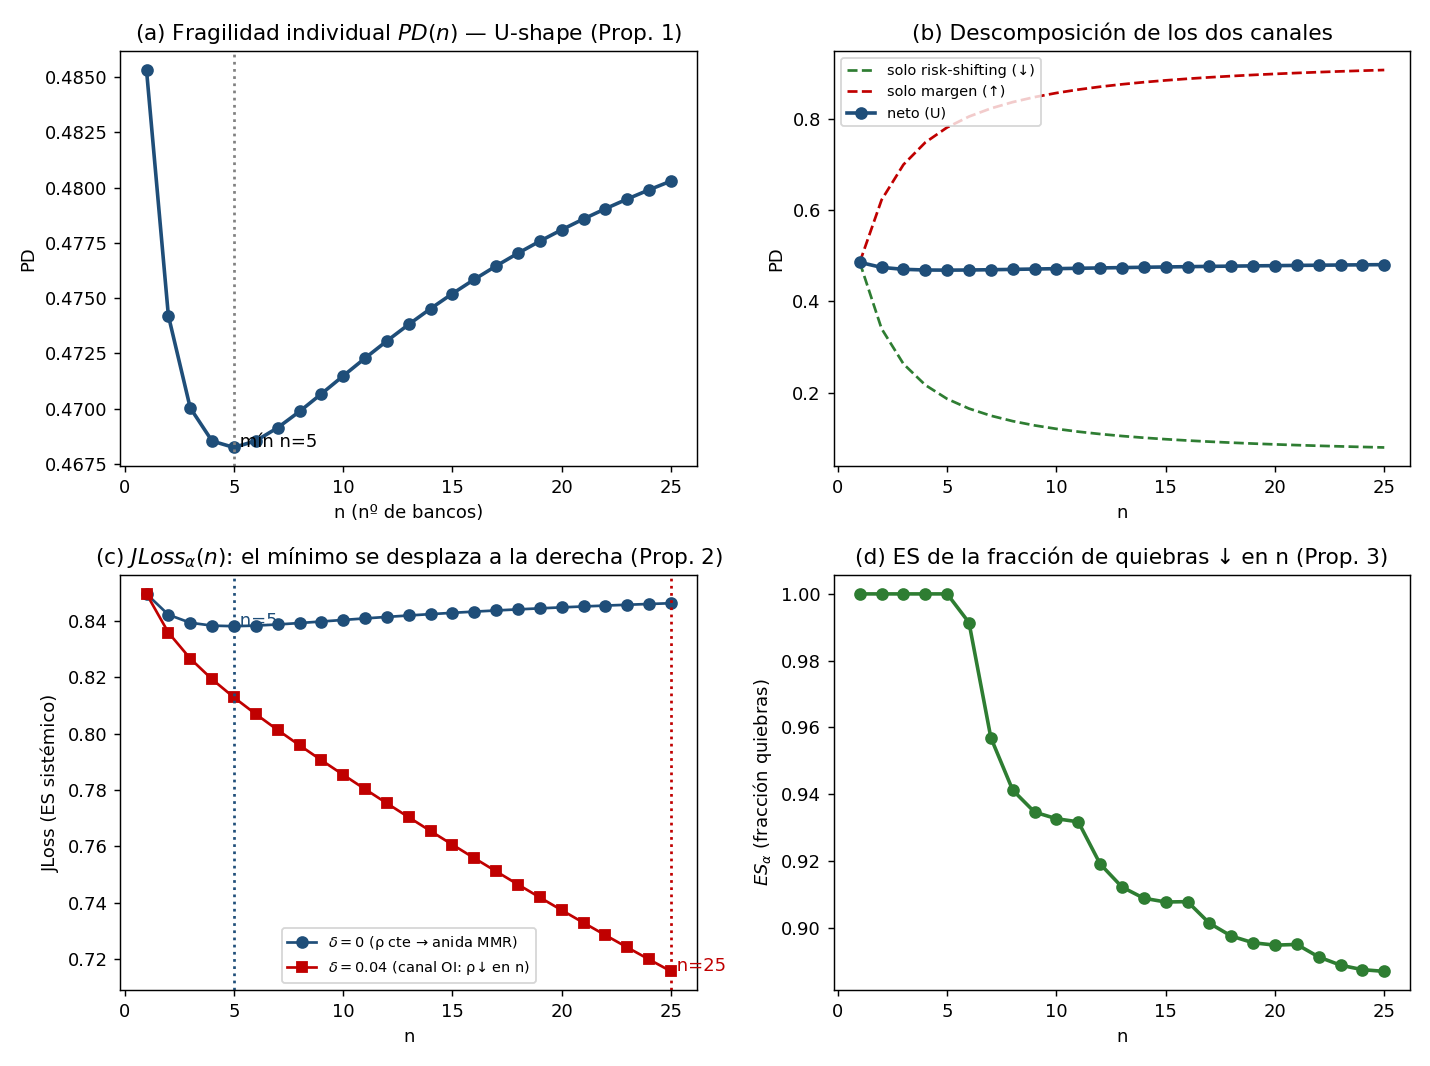
\includegraphics[width=0.95\textwidth]{fase3_calibracion.png}
\caption[Calibración del modelo Cournot--fragilidad]{Calibración del modelo. (a)~$\PD(n)$ en U; (b)~descomposición de canales; (c)~$\JLoss_\alpha(n)$ con mínimo desplazado a la derecha (Prop.~\ref{prop:shift}); (d)~$\ES$ de la fracción de quiebras, decreciente en $n$ (Prop.~\ref{prop:granular}). Los rótulos internos de los paneles reproducen la numeración del \textit{working paper} de origen; en la numeración de esta tesis corresponden a las Proposiciones~\ref{prop:U} (panel~a), \ref{prop:shift} (panel~c) y \ref{prop:granular} (panel~d).}
\label{fig:cal}
\end{figure}

\section{Cierre macro-soberano}\label{sec:soberano}

Los canales se derivan sobre el propio \textit{Growth-at-Risk} $\GaR_\tau$ (el cuantil bajo del crecimiento, negativo en la cola), por comodidad algebraica. Para que los signos coincidan con los de las regresiones del Capítulo~\ref{chap:paper2} y de los \texttt{.Rmd} del panel —que reportan la interacción sobre el \textbf{riesgo de cola} $D\equiv-\GaR$ (un $D$ mayor = cola más adversa)— el mapeo final (Sección~\ref{sec:empirico}) reexpresa los coeficientes en esa convención, con $\beta_3^{D}=-\beta_3^{\GaR}$ y $\beta_4^{D}=-\beta_4^{\GaR}$. La predicción de complementariedad es $\beta_3>0$ en convención $D$ (equivalentemente $\theta=\beta_3^{\GaR}<0$).

\subsection{Canal I: \texorpdfstring{$\JLoss\to\GaR$}{JLoss a GaR}}
La pérdida sistémica contrae el crédito ($K=\bar K-\phi L_{\text{sys}}$) y desplaza a la baja el cuantil del crecimiento:
\begin{equation}
\GaR_\tau=\mu-\Lambda(\JLoss)\ \Longrightarrow\ \partial\GaR_\tau/\partial\JLoss=-\Lambda'(\JLoss)<0,
\label{eq:gar}
\end{equation}
con $\partial\Lambda/\partial H>0$ (corolario macro de la Proposición~\ref{prop:granular}): el traspaso es más profundo en sistemas concentrados.

\subsection{Canal II: \texorpdfstring{$\GaR,\JLoss\to\Spread$}{GaR, JLoss al spread} y el \textit{doom loop}}
El spread compensa la pérdida esperada, $\Spread\approx LGD_{\text{sov}}\cdot\PD_{\text{sov}}$. La deuda proyectada en el estado malo es $d'=\frac{1+r}{1+g}d+B(\JLoss;H)/Y$, donde el crecimiento de cola es el propio \textit{Growth-at-Risk}, $g=\GaR_\tau$, y el costo de rescate $B$ es creciente en $\JLoss$ y en $H$. El soberano incumple si un choque fiscal $\eta$ supera la distancia al límite fiscal $DFL=\bar d-d'$ \citep{GhoshEtAl2013}, de modo que $\Spread=LGD_{\text{sov}}(1-F_\eta(DFL))$. Como $\partial DFL/\partial\GaR=+(1+r)d/(1+\GaR)^2>0$ (mejor crecimiento de cola, más espacio fiscal), se sigue $\partial\Spread/\partial\GaR<0$.

\begin{proposition}[complementariedad y amplificación estructural]\label{prop:cross}
Con $F_\eta$ unimodal y el punto de operación en la cola ($f_\eta'(DFL)<0$),
\[
\frac{\partial^2\Spread}{\partial\JLoss\,\partial \GaR}=LGD_{\text{sov}}\frac{B'_{\JLoss}}{Y}\,\underbrace{f_\eta'(DFL)}_{<0}\,\underbrace{\frac{\partial DFL}{\partial \GaR}}_{>0}<0
\;\Longleftrightarrow\;
\frac{\partial^2\Spread}{\partial\JLoss\,\partial D}>0,\qquad D\equiv-\GaR,
\]
es decir, fragilidad sistémica y riesgo a la baja son complementarios: el efecto marginal de $\JLoss$ sobre el spread \emph{crece} cuando el riesgo de cola $D$ sube (crecimiento de cola más adverso). Además la interacción se intensifica con la concentración, $\partial^3\Spread/(\partial\JLoss\,\partial D\,\partial H)>0$. (La demostración completa está en el Anexo~\ref{chap:anexoA}.)
\end{proposition}

\begin{remark}[la derivada cruzada no depende del Canal I]\label{rem:decouple}
La Proposición~\ref{prop:cross} se obtiene tratando $\JLoss$ y $D$ como argumentos
\emph{separados} de $\Spread$: $\JLoss$ entra por el costo de rescate $B(\JLoss;H)$ y
$D$ por el servicio de deuda proyectado $d'$. El signo del cross-partial no requiere
el Canal~I ($\JLoss\to\GaR$): aun si la fragilidad bancaria y el riesgo de cola del
crecimiento se determinaran de forma independiente, su coincidencia elevaría el
spread de forma supra-aditiva por la curvatura de $F_\eta$ en el punto de operación.
El Canal~I es un eslabón \emph{auxiliar} —que además cuenta con respaldo empírico
directo en la literatura de \textit{growth-at-risk} y de efectos reales de las
contracciones de crédito bancario \citep{ABG2019,Chari2024}— y no una premisa de la
complementariedad. El objeto firmado del modelo es la derivada cruzada.
\end{remark}

La Figura~\ref{fig:embi} ilustra el resultado: el panel~(a) muestra que la pendiente (negativa) de $\Spread$ respecto de $\GaR$ se empina con $\JLoss$ (complementariedad; en convención $D=-\GaR$, $\beta_3>0$), y el panel~(b), que el cross-partial se hace más pronunciado al aumentar la concentración ($\beta_4>0$ en convención $D$). La amplificación es un resultado \textit{local}: satura cuando $\PD_{\text{sov}}\to 1$.

\begin{figure}[t]
\centering
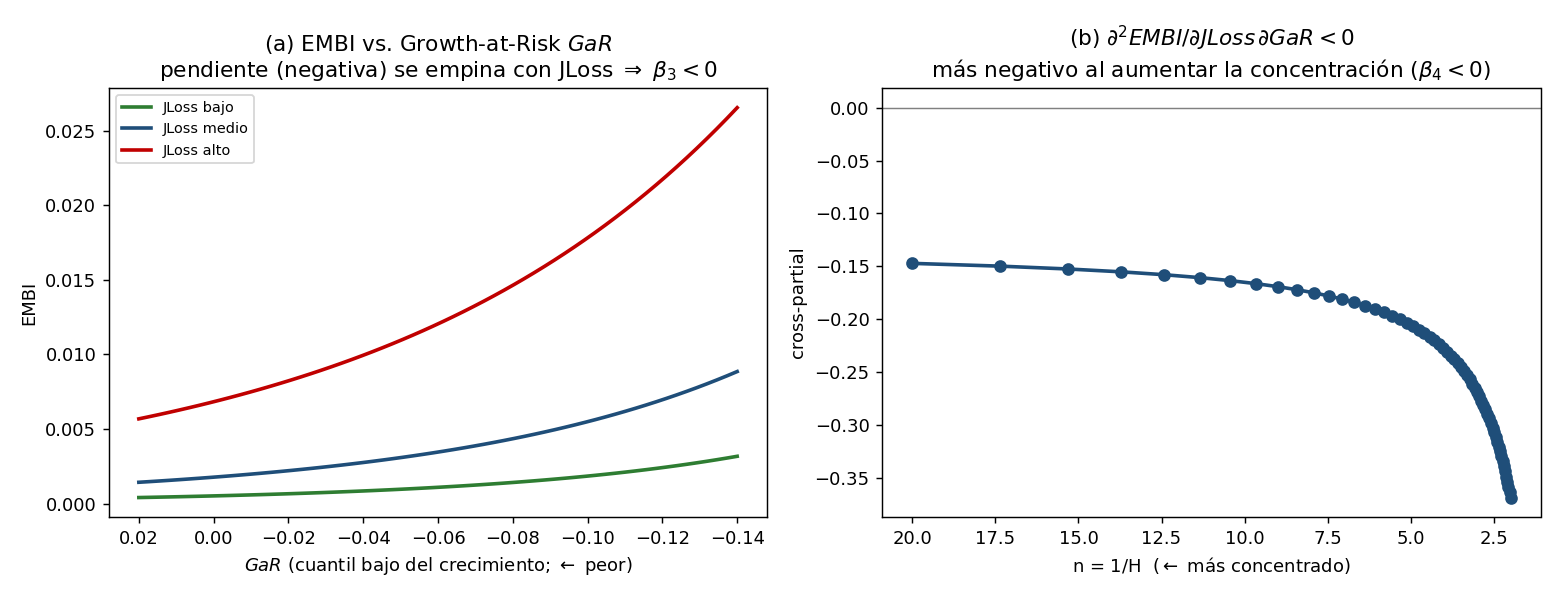
\includegraphics[width=0.95\textwidth]{fase4_embi.png}
\caption[Cierre soberano: complementariedad y amplificación]{Cierre soberano. (a)~$\Spread$ vs.\ $\GaR$ para tres niveles de $\JLoss$: la pendiente negativa se empina con $\JLoss$ (complementariedad; $\Rightarrow\beta_3>0$ en la convención $D\equiv-\GaR$, equiv.\ $\theta<0$ en convención $\GaR$); (b)~cross-partial más pronunciado al aumentar la concentración ($\Rightarrow\beta_4>0$ en convención $D$, Prop.~\ref{prop:cross}).}
\label{fig:embi}
\end{figure}

\section{Estrategia empírica}\label{sec:empirico}

\subsection{Especificación e hipótesis}
La cadena teórica entrega la especificación de panel con efectos fijos bidireccionales:
\begin{multline}
\Spread_{i,t}=\alpha_i+\delta_t+\beta_1\JLoss_{i,t}+\beta_2^{D} D_{i,t}+\beta_3(\JLoss\times D)_{i,t}\\
{}+\beta_4(\JLoss\times D\times\HHI)_{i,t}+\boldsymbol{\varphi}'\,\mathrm{Int}_{i,t}+\boldsymbol{\gamma}'X_{i,t}+\varepsilon_{i,t},\qquad D_{i,t}\equiv-\GaR_{i,t},
\label{eq:emp}
\end{multline}
donde $\mathrm{Int}_{i,t}$ recoge las interacciones de orden inferior que la triple interacción arrastra por construcción ($\JLoss\times\HHI$ y $D\times\HHI$) y $X_{i,t}$ el vector de controles. Las predicciones firmadas son $\beta_1>0$, $\beta_2^{D}>0$ (equivalentemente $\beta_2<0$ en convención $\GaR$), $\beta_3>0$ (complementariedad, Prop.~\ref{prop:cross}) y $\beta_4>0$ (amplificación por concentración). Se usa el riesgo de cola $D\equiv-\GaR$ —como en el Capítulo~\ref{chap:paper2} y en las regresiones del panel— de modo que un coeficiente \emph{positivo} sobre el producto refuerza el spread cuando la fragilidad y el riesgo de cola empeoran simultáneamente; en la parametrización con $\GaR$, los signos son $\theta=\beta_3^{\GaR}<0$ y $\beta_4^{\GaR}<0$. Las hipótesis intermedias son la U de la fragilidad (Prop.~\ref{prop:U}), el mínimo desplazado de $\JLoss$ (Prop.~\ref{prop:shift}) y el traspaso $\JLoss\to\GaR$ creciente en concentración por regresión cuantílica (Prop.~\ref{prop:granular}).

\subsection{Qué estima cada coeficiente}\label{sec:estimandos}
Conviene fijar, para cada $\beta_k$ de \eqref{eq:emp}, el objeto estructural que le
corresponde y el estimando poblacional que recupera bajo los supuestos de
identificación (Cuadro~\ref{tab:estimandos}). Dos precisiones importan para la
interpretación. Primera: como $\GaR$ (vía $D$) entra en la ecuación, $\beta_1$ es el
efecto \emph{directo} de $\JLoss$ sobre el spread, \emph{neto} del canal de
\textit{credit crunch}; el efecto \emph{total} de la fragilidad es
$\beta_1+\beta_2^{D}\,(\partial D/\partial\JLoss)$, con
$\partial D/\partial\JLoss>0$ por el Canal~I. Segunda: $\JLoss$ y $\GaR$ son
\emph{regresores generados} —el primero por el motor Merton/punto de silla, el
segundo por regresión cuantílica—, de modo que la inferencia que los trata como
datos subestima la varianza de $\hat\beta_k$; el Capítulo~\ref{chap:paper2} acota
ese sesgo por perturbación del regresor y muestra que el error de medición
\emph{atenúa} $\hat\beta_3$ hacia cero.

\begin{table}[t]
\centering
\small
\begin{tabular}{@{}p{1.3cm}p{3.0cm}p{7.6cm}@{}}
\toprule
Coef. & Término & Estimando (bajo EF país$+$tiempo, exogeneidad condicional) \\
\midrule
$\beta_1$ & $\JLoss$ & Efecto marginal directo de la fragilidad sobre el spread, manteniendo $D$ fijo; \emph{no} incluye la parte mediada por el Canal~I. \\
$\beta_2^{D}$ & $D\equiv-\GaR$ & Efecto del riesgo de cola sobre el spread manteniendo $\JLoss$ fijo (canal de límite fiscal puro). \\
$\beta_3$ & $\JLoss\times D$ & $E\!\left[\partial^2\Spread/\partial\JLoss\,\partial D\mid \alpha_i,\delta_t\right]$: cuánto crece el efecto marginal de $\JLoss$ por punto de $D$ (complementariedad, Prop.~\ref{prop:cross}). \\
$\beta_4$ & $\JLoss\times D\times\HHI$ & $E\!\left[\partial^3\Spread/\partial\JLoss\,\partial D\,\partial\HHI\right]$: cómo cambia $\beta_3$ con la concentración; identificado \emph{de la varianza transversal de $\HHI$}, por lo que con trece países es impreciso (Sección~\ref{sec:datos_reales}). \\
\bottomrule
\end{tabular}
\caption[Objeto estructural y estimando de cada coeficiente]{Objeto estructural y estimando de cada coeficiente de \eqref{eq:emp}. Todos los signos en convención $D\equiv-\GaR$.}
\label{tab:estimandos}
\end{table}

\subsection{Identificación}
El desafío es la simultaneidad del \textit{doom loop}. La estrategia es escalonada: (i)~efectos fijos país y tiempo con regresores rezagados y errores estándar de Driscoll--Kraay; (ii)~instrumentos de competencia (choques de entrada/desregulación, Sección~\ref{sec:npolitica}) si hay simultaneidad; (iii)~proyecciones locales para la respuesta dinámica. La inferencia se concentra en $\beta_4$, menos contaminada por la retroalimentación de nivel porque la heterogeneidad opera sobre $\HHI$ predeterminado a nivel país.

\subsection{El DAG del mecanismo}\label{sec:dag}
La Figura~\ref{fig:dag} resume la estructura causal. La \emph{cadena estructural}
(columna izquierda) va de la política de competencia al spread por los canales que
las Secciones~\ref{sec:sistemico}--\ref{sec:soberano} derivan. Sobre ella operan dos
conjuntos de \emph{causas comunes}: el factor macro-financiero global $Z$ —tasas de
EE.UU., aversión al riesgo, VIX— incide a la vez sobre $\JLoss$ y sobre $\GaR$ y es
el origen de la correlación positiva y moderada entre ambos (aproximadamente $+0{,}2$
en convención $D$); los fundamentos domésticos $X_{i,t}$ inciden sobre la fragilidad,
la cola del crecimiento y el spread. Los efectos fijos de tiempo absorben $Z$ y los
de país absorben la parte invariante de $X_{i,t}$; el vector de controles absorbe su
parte variable. Quedan fuera del modelo las aristas de \emph{retroalimentación}
(línea punteada): el spread alto deprime el crecimiento y golpea los balances
bancarios, y una crisis induce consolidación. El cierre de un período trata esas
aristas como agenda (Sección~\ref{sec:conclusion}). El DAG deja ver el punto central
de la identificación de la interacción: $\JLoss$ llega al spread por un camino
($\JLoss\!\to\!B\!\to\!DFL\!\to\!\Spread$) que \emph{no} pasa por $\GaR$, y $\GaR$ por
otro ($\GaR\!\to\!d'\!\to\!DFL\!\to\!\Spread$) que no pasa por $\JLoss$ —son canales
distintos aun cuando el Canal~I exista (Observación~\ref{rem:decouple}).

\begin{figure}[t]
\centering
\shorthandoff{<>}% babel-spanish hace activos < y > (guillemets); tikz los necesita literales
\begin{tikzpicture}[
  >={Stealth[length=2mm]}, font=\footnotesize,
  node distance=7mm and 34mm,
  b/.style={draw, rounded corners=1.5pt, align=center, inner sep=3pt, minimum width=20mm, minimum height=6mm},
  c/.style={draw, dashed, rounded corners=1.5pt, align=center, inner sep=3pt, fill=black!4},
  lab/.style={font=\scriptsize, midway, fill=white, inner sep=1pt}
]
  \node[c] (pol) {política de entrada ($F$)};
  \node[b, below=of pol] (n) {$n$};
  \node[b, below=of n] (jl) {$\JLoss$};
  \node[b, below=of jl] (gar) {$\GaR$\;\;($D\!\equiv\!-\GaR$)};
  \node[b, below=of gar] (dfl) {$DFL=\bar d-d'$};
  \node[b, below=of dfl] (sp) {$\Spread$};

  \draw[->] (pol) -- (n);
  \draw[->] (n)  -- node[lab]{$\rho(n),R_L^*,\PD,H$} (jl);
  \draw[->] (jl) -- node[lab]{Canal I: $\Lambda(\JLoss;H)$} (gar);
  \draw[->] (gar)-- node[lab]{$d'(\GaR)$} (dfl);
  \draw[->] (dfl)-- node[lab]{$1-F_\eta(\cdot)$} (sp);
  \draw[->] (jl.west) to[out=195,in=165,looseness=1.35]
        node[lab, pos=0.1, left=1pt]{$B(\JLoss;H)$} (dfl.west);

  \node[c, right=of jl] (Z) {$Z$, factores globales\\{\scriptsize(EF de tiempo)}};
  \node[c, right=of dfl] (X) {fundamentos $X_{i,t}$\\{\scriptsize(EF de país + controles)}};
  \draw[->, dashed] (Z) -- (jl);
  \draw[->, dashed] (Z.south) to[out=250,in=25] (gar.east);
  \draw[->, dashed] (X) -- (dfl);
  \draw[->, dashed] (X.south) to[out=280,in=25] (sp.east);

  \draw[->, dotted] (sp.south) to[out=340,in=345,looseness=2.6]
        node[lab, pos=0.5, right=1pt]{retroalimentación} (jl.east);
\end{tikzpicture}
\shorthandon{<>}%
\caption[El DAG del mecanismo]{Estructura causal del modelo. Cadena estructural
(cajas sólidas); causas comunes absorbidas por los efectos fijos (cajas
discontinuas); aristas de retroalimentación no modeladas (punteado). $\JLoss$ y
$\GaR$ alcanzan el spread por caminos que no se cruzan, de modo que $\beta_1$ y
$\beta_2^{D}$ identifican canales distintos.}
\label{fig:dag}
\end{figure}

\subsection{Validación del diseño por Monte Carlo}
Antes de estimar con datos reales se verificó que la especificación \eqref{eq:emp} recupera los efectos teóricos. Se simuló un panel desde el modelo estructural y se estimó por TWFE con errores estándar agrupados por país, sobre $R=3000$ réplicas. En la convención $D\equiv-\GaR$ de \eqref{eq:emp} los valores verdaderos son $\beta_3=+0{,}80$ y $\beta_4=+3{,}0$ (el mismo experimento en convención $\GaR$ tiene $\beta_3=-0{,}80$, $\beta_4=-3{,}0$: multiplicar el regresor por $-1$ invierte exactamente el coeficiente). Con $N=45$, $T=80$, las medias son $\hat\beta_3=+0{,}799$ y $\hat\beta_4=+3{,}001$ ---prácticamente insesgadas---, del signo predicho en el \textbf{100\%} de las réplicas, con potencia del 93\% al 5\% (Figura~\ref{fig:mc}). El OLS agrupado sin efectos fijos sesga fuertemente la triple interacción, lo que confirma la necesidad de los efectos fijos bidireccionales. Un barrido de tamaño muestral muestra que la potencia de $\beta_4$ crece monótonamente con los datos, de $\sim$24\% con 600 observaciones a $\sim$99\% con 6000, de modo que la potencia moderada de paneles cortos se resuelve ampliando la cobertura de países y la ventana temporal.

\begin{figure}[t]
\centering
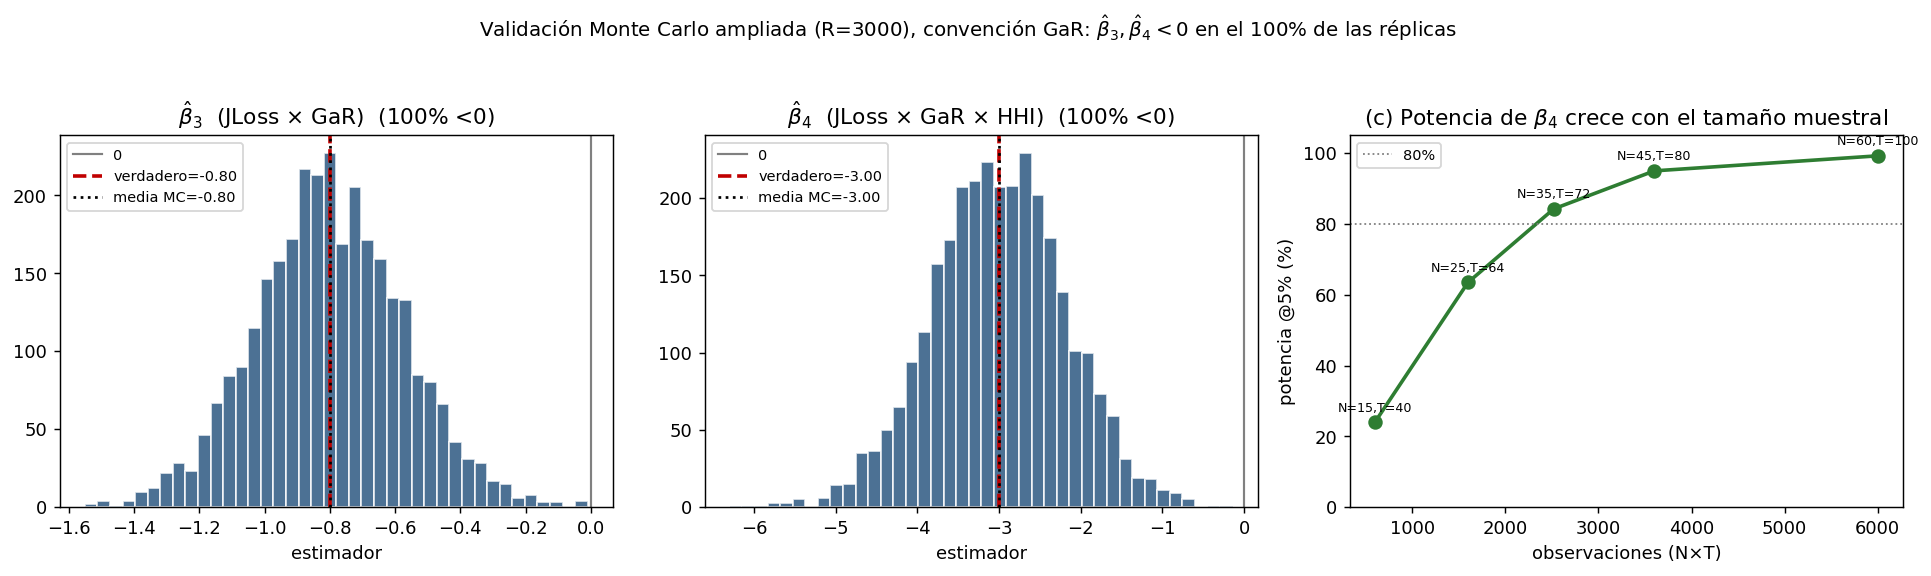
\includegraphics[width=0.95\textwidth]{fase5_montecarlo.png}
\caption[Validación Monte Carlo del diseño empírico]{Validación Monte Carlo ampliada ($R=3000$, $N=45$, $T=80$). El gráfico se generó en convención $\GaR$ ($\beta_3,\beta_4<0$); en la convención $D\equiv-\GaR$ de \eqref{eq:emp} las distribuciones son idénticas con el signo invertido ($\beta_3=+0{,}80$, $\beta_4=+3{,}0$ verdaderos). (a)--(b)~distribución muestral de $\hat\beta_3$ y $\hat\beta_4$: insesgada en media y del mismo signo en el 100\% de las réplicas; (c)~la potencia de $\beta_4$ crece con el tamaño muestral.}
\label{fig:mc}
\end{figure}

\subsection{Estimación con datos reales: H4a y H4b}\label{sec:datos_reales}

La validación Monte Carlo de la sección anterior confirma que la especificación \eqref{eq:emp} recupera correctamente los parámetros de un modelo cuya verdad se conoce por construcción. El paso decisivo --y el que distingue a este trabajo de un ejercicio puramente deductivo-- es contrastar las dos predicciones firmadas y distintivas del modelo, H4a (complementariedad) y H4b (amplificación por concentración), contra el panel real de economías emergentes construido para el Capítulo~\ref{chap:paper2}: $\JLoss$ estimado por el método de punto de silla sobre balances bancarios y precios accionarios de Bloomberg, $\GaR$ por regresión cuantílica de panel sobre condiciones financieras observadas, el spread soberano medido por el EMBI Global Diversified, y $\HHI$ aproximado por la concentración estructural de los tres bancos mayores (\textit{World Bank Global Financial Development Database}, GFDD), con la serie anual del mismo indicador como robustez.

\paragraph{H4a: la complementariedad.} Sobre el panel único de trece economías emergentes (Capítulo~\ref{chap:paper2}, Sección 5), el coeficiente de interacción de la especificación de nivel tiene el signo predicho pero no es significativo sobre la muestra completa ($\hat\beta_3=+0{,}16$, $p=0{,}26$; en convención $\GaR$, $\hat\theta=-0{,}16$). El Capítulo~\ref{chap:paper2} muestra que esa no significancia es \textbf{condicional}: la interacción sí es significativa ($\hat\beta_3=+0{,}47$, $t=2{,}29$, $p=0{,}023$) sobre el núcleo de once economías emergentes de financiamiento externo, y se diluye al añadir Polonia e India, dos economías con mercados de deuda local profundos —aunque, con solo dos economías en el grupo de contraste, la diferencia entre grupos no alcanza significancia estadística formal. Un modelo de umbral de panel corrobora la no linealidad (efecto de la fragilidad unas tres veces mayor en el régimen de cola severa). H4a es, por tanto, una regularidad de \textbf{signo y forma} respaldada de manera condicional —presente en las economías más expuestas al financiamiento externo—, no una regularidad universal. En la parametrización con la triple interacción (el término $\beta_3$ de \eqref{eq:emp}, estimado \emph{junto con} $\JLoss\times D\times\HHI$ y con $\HHI$ centrado) $\hat\beta_3$ \textbf{no está identificado}: sale con el signo predicho pero no significativo con los dos proxies de concentración del GFDD ($+32{,}5$ y $+23{,}3$, $|t|<0{,}6$) y no distinguible de cero con la concentración trimestral ($-4{,}0$, $t=-0{,}12$). El contraste con potencia de H4a es el término $\JLoss\times D$ sin $\HHI$ (arriba).

\paragraph{H4b: la amplificación por concentración --- no identificada.} La predicción que distingue a este modelo de \citet{MMR2010} --que la propia complementariedad $\JLoss\times\GaR$ se intensifica en sistemas bancarios más concentrados-- se contrasta incorporando la triple interacción $\JLoss\times D\times\HHI$ (con $D\equiv-\GaR$). Sobre el panel anclado en Bloomberg, esta predicción \textbf{no puede contrastarse con potencia}: en la parametrización de nivel $D\equiv-\GaR$ (donde la predicción es $\beta_4>0$), el punto estimado de $\hat\beta_4$ es pequeño y muy impreciso con los tres proxies de concentración —$+139$ ($t=0{,}39$) con el $\HHI$ estructural del GFDD, $+171$ ($t=0{,}81$) con la serie anual, y $\approx 0$ ($t=-0{,}54$) con la concentración trimestral— y en los tres casos el \textit{bootstrap} de bloques por país deja el intervalo de confianza al 90\% cruzando el cero holgadamente ($P(\hat\beta_4>0)$ entre 43\,\% y 68\,\%). Con trece \textit{clusters} de país y un $\HHI$ casi invariante en el tiempo, el coeficiente \textbf{no está identificado}: no respalda ni refuta la predicción. La propia validación Monte Carlo lo anticipa: la potencia de $\beta_4$ crece de $\sim$24\% con 600 observaciones a $\sim$99\% con 6000, de modo que el efecto mínimo detectable sobre una muestra de este orden es varias veces la magnitud calibrada. H4b queda, por tanto, como una \textbf{predicción registrada del modelo} cuyo contraste con potencia exige un corte transversal sustancialmente más amplio; la prueba con potencia que sí ofrece este capítulo es la de H4a, el término $\JLoss\times D$ sin $\HHI$. Para descartar que el problema sea únicamente la falta de variación temporal del proxy del GFDD, se construyó además una concentración \textbf{trimestral} a partir de los mismos balances bancarios de Bloomberg que alimentan $\JLoss$ (activos de los tres mayores bancos cotizados sobre el total cotizado, por país y trimestre; correlación de $0{,}48$ con el GFDD anual). Con esa serie el resultado tampoco cambia: el intervalo robusto cruza el cero. Contrasta con la reconstrucción previa basada en datos regulatorios, en la que $\hat\beta_4=+721$ ($t=2{,}98$) sí confirmaba la predicción sobre una serie de fragilidad de dispersión transversal mucho mayor (Figura~\ref{fig:h4b}); la discrepancia se discute a continuación.

\begin{figure}[t]
\centering
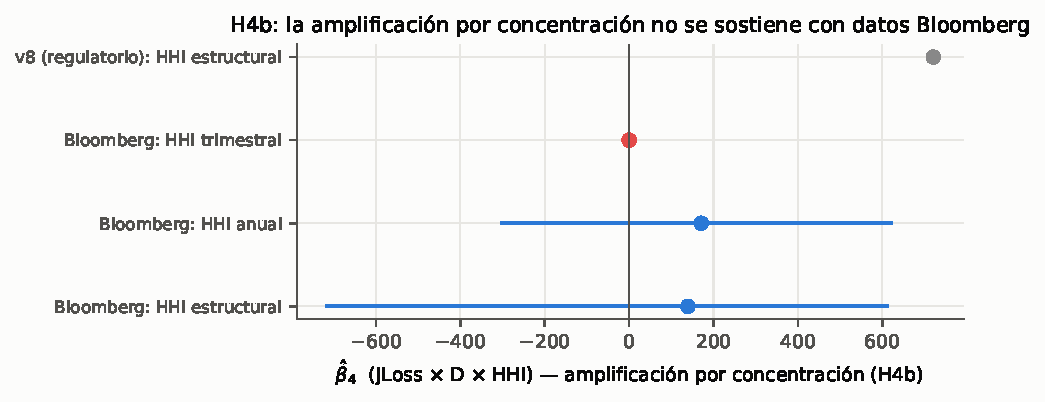
\includegraphics[width=0.9\textwidth]{fig_h4b.pdf}
\caption[Amplificación por concentración: regulatorio vs.\ Bloomberg]{Coeficiente de amplificación por concentración $\hat\beta_4$ (parametrización de nivel $D\equiv-\GaR$, donde $\beta_4>0$ es la predicción del modelo). Barras: IC 90\% (\textit{bootstrap} de bloques por país). El punto gris reproduce la estimación con datos regulatorios ($+721$, significativa); sobre el panel homogéneo de Bloomberg el intervalo cruza el cero con todos los proxies de concentración.}
\label{fig:h4b}
\end{figure}

\paragraph{Interpretación.} Tres explicaciones, no excluyentes, dan cuenta de la diferencia respecto de la versión regulatoria, en la que $\hat\beta_4$ era significativa y del signo predicho. \emph{Primera}, y la más probable: la serie de $\JLoss$ construida homogéneamente desde Bloomberg es transversalmente mucho más comprimida (desviación estándar $\approx$4,6, frente a 8,3 en la versión regulatoria, donde Brasil concentraba una fragilidad medida $\approx$16). La triple interacción $\JLoss\times D\times\HHI$ necesita covariación entre países de la fragilidad \emph{y} de la concentración; al homogeneizar la métrica se elimina buena parte de la dispersión de $\JLoss$ sobre la que descansaba el $+721$ regulatorio, que —a la luz de esto— pudo haber sido un artefacto de la enorme fragilidad medida de un solo país. \emph{Segunda}: el proxy de concentración del GFDD es casi invariante en el tiempo, de modo que $\beta_4$ se identifica esencialmente de un puñado de valores transversales de $\HHI$ --potencia que la propia validación Monte Carlo anticipaba en 60--70\% con muestras de este orden. Esta segunda explicación se puso a prueba directamente construyendo la concentración trimestral descrita arriba: con variación temporal genuina el coeficiente \emph{sigue sin identificarse} (el intervalo de bloques cruza el cero), lo que descarta que la falta de variación temporal del proxy sea, por sí sola, la explicación completa. \emph{Tercera}: el canal de amplificación por granularidad y correlación (Proposiciones~\ref{prop:granular}--\ref{prop:cross}) podría ser genuinamente más débil de lo que sugiere la calibración del modelo. Con las dos primeras explicaciones parcialmente descartadas por los datos, la tercera gana peso relativo; distinguirla con precisión requiere un universo de países más amplio. \textbf{La predicción distintiva del modelo no puede contrastarse con potencia sobre los datos homogéneos disponibles}, y la contribución empírica de este capítulo se reduce a H4a --la complementariedad de primer orden, cuyo signo y forma se sostienen de forma condicional (en el núcleo de economías de financiamiento externo) según reporta el Capítulo~\ref{chap:paper2}.

\section{Robustez y revisión adversarial}\label{sec:robustez}

\subsection{Extensión à la Salop y microfundamento de \texorpdfstring{$\rho(n)$}{rho(n)}}
Bajo competencia espacial de Salop, el margen de equilibrio es $m^*(n)=t/n$ y la libre entrada fija $n^*=\sqrt{t/F}$, decreciente en la barrera de entrada $F$. Las Proposiciones~\ref{prop:U}--\ref{prop:cross} se preservan, y la mayor diferenciación con más bancos \textit{microfundamenta} $\rho'(n)<0$. Esto entrega una predicción nueva: mayores barreras de entrada implican más concentración y, por tanto, mayor riesgo sistémico y mayor amplificación del spread (Figura~\ref{fig:rob}b). El supuesto $\rho'(n)<0$ compite con un canal de \textit{herding} \citep{AcharyaYorulmazer2007} que podría revertirlo; el modelo entrega la condición de dominancia y traslada el signo al dato.

\subsection{Validación del método de cálculo de \texorpdfstring{$\JLoss$}{JLoss}}
La Figura~\ref{fig:rob}a valida la cola de la pérdida sistémica con exposiciones heterogéneas: la convolución exacta coincide con Monte Carlo, y la aproximación de punto de silla es precisa en la cola profunda (el rango relevante para $\ES/VaR$) aunque se degrada en el cuerpo cuando la cartera es muy granular. Se recomienda convolución/Monte Carlo para sistemas concentrados y punto de silla para carteras grandes.

\begin{figure}[t]
\centering
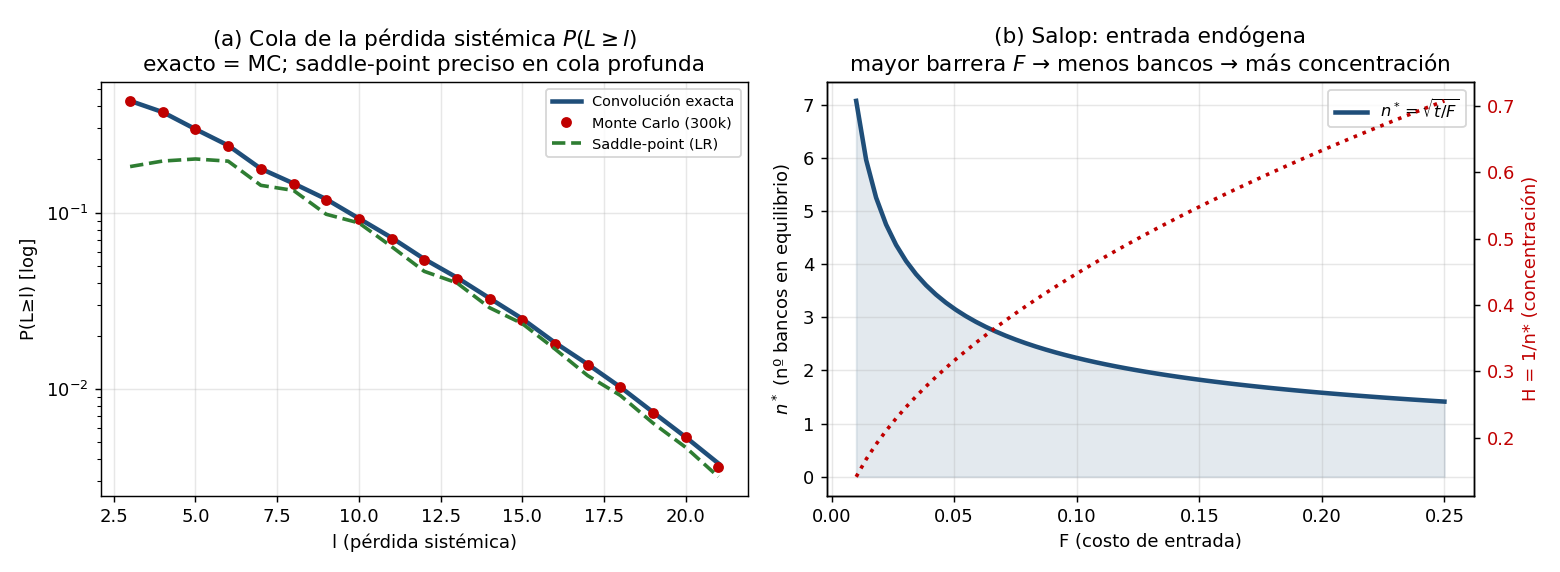
\includegraphics[width=0.95\textwidth]{fase6_robustez.png}
\caption[Robustez: cola de la pérdida sistémica y entrada Salop]{Robustez. (a)~Validación de la cola de $L$: convolución exacta = Monte Carlo; punto de silla preciso en la cola profunda. (b)~Salop: $n^*=\sqrt{t/F}$ decreciente en la barrera de entrada.}
\label{fig:rob}
\end{figure}

\subsection{Coherencia con hechos estilizados}
La relación en U (Prop.~\ref{prop:U}) reconcilia la evidencia contradictoria: \citet{BeckDemirgucLevine2006} hallan que sistemas concentrados sufren menos crisis, mientras que otros hallan lo contrario; el signo observado depende del tramo de competencia de cada muestra. La distinción entre riesgo individual y sistémico (Prop.~\ref{prop:shift}) explica por qué estudios sobre quiebras individuales y sobre crisis sistémicas llegan a conclusiones distintas.

\subsection{Límites reconocidos}
Una revisión adversarial explícita identifica los límites del modelo: la U es poco profunda (rasgo conocido de \citealp{MMR2010}, pero el canal $\rho$ no depende de su profundidad); el bloque soberano es de equilibrio parcial (el lazo completo requiere dinámica de dos períodos); el cross-partial es un resultado local que satura; y la identificación empírica enfrenta simultaneidad y potencia moderada. Sobre este último punto, conviene ser específico: la Sección~\ref{sec:empirico} anuncia \textit{instrumentos de competencia} (choques de entrada o desregulación) como vía para resolver la simultaneidad del \textit{doom loop} si esta se manifestara, pero esa estrategia \textbf{no llegó a implementarse} —H4a y H4b se estiman por efectos fijos bidireccionales y \textit{bootstrap} de bloques, no por variables instrumentales—, de modo que la simultaneidad del lazo soberano-bancario no está cerrada en este capítulo. La dificultad no es hipotética: el Capítulo~\ref{chap:paper2} sí intenta instrumentar el nivel de $\JLoss$ —el mismo objeto que la simultaneidad de este capítulo pondría en duda— y la estrategia de variables instrumentales no cierra la identificación (primera etapa apenas aceptable, un segundo instrumento con signo opuesto y rechazo del test de sobre-identificación). Esa dificultad documentada para instrumentar $\JLoss$ en el capítulo hermano es motivo adicional de cautela sobre cuán fácil sería, en la práctica, construir el instrumento de competencia que aquí se menciona solo como posibilidad. Estas limitaciones se documentan con vías de mitigación en lugar de ocultarse.

\section{Conclusión del capítulo}\label{sec:conclusion}

Este capítulo muestra que la estructura de mercado bancario es un determinante profundo, y hasta ahora subestimado, de la cadena que va desde la fragilidad sistémica hasta el riesgo soberano. Al distinguir el riesgo individual del riesgo de cola conjunta y endogenizar la correlación de activos, el modelo genera una predicción distinguible de la literatura estándar: el mercado que minimiza el riesgo sistémico es más competido que el que minimiza el riesgo individual, y la concentración amplifica la transmisión de la fragilidad al spread soberano cuando el crecimiento está en la cola.

Las predicciones no quedan solo como ejercicio deductivo. Contrastadas mediante la especificación \eqref{eq:emp} sobre un único panel de trece economías emergentes, con la fragilidad bancaria anclada en Bloomberg y el spread medido por el EMBI Global Diversified (Sección~\ref{sec:datos_reales}), el resultado es asimétrico. La complementariedad $\JLoss\times D$ (H4a; $D\equiv-\GaR$) tiene el signo y la forma predichos —corroborados por un modelo de umbral que no impone la forma funcional de la interacción— con significancia \textbf{condicional}: se sostiene sobre el núcleo de once economías emergentes de financiamiento externo y se diluye al añadir economías con mercados de deuda local profundos, sin que la diferencia entre grupos, con solo dos economías en el segundo, alcance un contraste formal. La predicción que distingue a este modelo de \citet{MMR2010}, la amplificación por la concentración bancaria (H4b), \textbf{no puede contrastarse con potencia sobre estos datos}: el punto estimado de la triple interacción no tiene signo estable entre proxies de concentración y su intervalo de confianza robusto cruza el cero con todos ellos, incluida una serie \textbf{trimestral} construida de los mismos balances Bloomberg que $\JLoss$ —lo que descarta que la falta de variación temporal del proxy sea, por sí sola, la explicación. Este trabajo concluye, por tanto, que el eslabón teoría--evidencia de la cadena se sostiene para el mecanismo de primer orden en las economías más expuestas al financiamiento externo, pero \emph{queda abierto} para la heterogeneidad por concentración, con el peso de la evidencia inclinándose hacia un canal de amplificación genuinamente más débil que su calibración antes que hacia un artefacto de medición del proxy. La agenda pendiente --la dinámica de dos períodos del lazo soberano-bancario, el microfundamento completo de $\rho(n)$ más allá del caso Salop, y un universo de países más amplio-- es la vía directa para cerrar la pregunta.

\section*{Referencias del capítulo}
\addcontentsline{toc}{section}{Referencias del capítulo}

\begin{thebibliography}{99}
\sloppy\small
\bibitem[Acharya et al.(2017)]{AcharyaEtAl2017} Acharya, V., Pedersen, L., Philippon, T., Richardson, M. (2017). Measuring Systemic Risk. \textit{Review of Financial Studies} 30(1), 2--47.
\bibitem[Acharya et al.(2014)]{AcharyaDrechslerSchnabl2014} Acharya, V., Drechsler, I., Schnabl, P. (2014). A Pyrrhic Victory? Bank Bailouts and Sovereign Credit Risk. \textit{Journal of Finance} 69(6), 2689--2739.
\bibitem[Acharya \& Yorulmazer(2007)]{AcharyaYorulmazer2007} Acharya, V., Yorulmazer, T. (2007). Too Many to Fail. \textit{Journal of Financial Intermediation} 16(1), 1--31.
\bibitem[Adrian et al.(2019)]{ABG2019} Adrian, T., Boyarchenko, N., Giannone, D. (2019). Vulnerable Growth. \textit{American Economic Review} 109(4), 1263--1289.
\bibitem[Adrian \& Brunnermeier(2016)]{AdrianBrunnermeier2016} Adrian, T., Brunnermeier, M. (2016). CoVaR. \textit{American Economic Review} 106(7), 1705--1741.
\bibitem[Allen \& Gale(2004)]{AllenGale2004} Allen, F., Gale, D. (2004). Competition and Financial Stability. \textit{Journal of Money, Credit and Banking} 36(3), 453--480.
\bibitem[Beck et al.(2006)]{BeckDemirgucLevine2006} Beck, T., Demirgüç-Kunt, A., Levine, R. (2006). Bank Concentration, Competition, and Crises. \textit{Journal of Banking \& Finance} 30(5), 1581--1603.
\bibitem[Boyd \& De Nicoló(2005)]{BoydDeNicolo2005} Boyd, J., De Nicoló, G. (2005). The Theory of Bank Risk Taking and Competition Revisited. \textit{Journal of Finance} 60(3), 1329--1343.
\bibitem[Chan et al.(1992)]{ChanGreenbaumThakor1992} Chan, Y.S., Greenbaum, S., Thakor, A. (1992). Is Fairly Priced Deposit Insurance Possible? \textit{Journal of Finance} 47(1), 227--245.
\bibitem[Chari et al.(2024)]{Chari2024} Chari, A., Garcés, F., Martínez, J. F., Valenzuela, P. (2024). Sovereign Credit Spreads, Banking Fragility, and Global Factors. \textit{Journal of Financial Stability} 72, 101235.
\bibitem[Farhi \& Tirole(2018)]{FarhiTirole2018} Farhi, E., Tirole, J. (2018). Deadly Embrace: Sovereign and Financial Balance Sheets Doom Loops. \textit{Review of Economic Studies} 85(3), 1781--1823.
\bibitem[Ghosh et al.(2013)]{GhoshEtAl2013} Ghosh, A., Kim, J., Mendoza, E., Ostry, J., Qureshi, M. (2013). Fiscal Fatigue, Fiscal Space and Debt Sustainability. \textit{Economic Journal} 123(566), F4--F30.
\bibitem[Gordy(2003)]{Gordy2003} Gordy, M. (2003). A Risk-Factor Model Foundation for Ratings-Based Bank Capital Rules. \textit{Journal of Financial Intermediation} 12(3), 199--232.
\bibitem[Keeley(1990)]{Keeley1990} Keeley, M. (1990). Deposit Insurance, Risk, and Market Power in Banking. \textit{American Economic Review} 80(5), 1183--1200.
\bibitem[Martínez-Miera \& Repullo(2010)]{MMR2010} Martínez-Miera, D., Repullo, R. (2010). Does Competition Reduce the Risk of Bank Failure? \textit{Review of Financial Studies} 23(10), 3638--3664.
\bibitem[Merton(1974)]{Merton1974} Merton, R. (1974). On the Pricing of Corporate Debt. \textit{Journal of Finance} 29(2), 449--470.
\bibitem[Merton(1977)]{Merton1977} Merton, R. (1977). An Analytic Derivation of the Cost of Deposit Insurance and Loan Guarantees. \textit{Journal of Banking \& Finance} 1(1), 3--11.
\bibitem[Stiglitz \& Weiss(1981)]{StiglitzWeiss1981} Stiglitz, J., Weiss, A. (1981). Credit Rationing in Markets with Imperfect Information. \textit{American Economic Review} 71(3), 393--410.
\bibitem[Vasicek(2002)]{Vasicek2002} Vasicek, O. (2002). The Distribution of Loan Portfolio Value. \textit{Risk} 15(12), 160--162.
\bibitem[Vives(2016)]{Vives2016} Vives, X. (2016). \textit{Competition and Stability in Banking}. Princeton University Press.
\end{thebibliography}


\appendix
\chapter{Apéndice matemático: demostraciones detalladas paso a paso}
\label{chap:anexoA}

\noindent Este anexo detalla, paso a paso, cada derivada y conclusión matemática del modelo del Capítulo~\ref{chap:paper1}. Se usa el \emph{Growth-at-Risk} $\GaR_\tau$ como variable primitiva ---el cuantil bajo del crecimiento, negativo en la cola--- de modo que los signos derivados del modelo coinciden \emph{directamente} con los de las regresiones del Capítulo~\ref{chap:paper2}, sin ningún cambio de variable intermedio: $\beta_1>0$, $\beta_2<0$, $\beta_3<0$, $\beta_4<0$. Todas las identidades (incluidas la derivada cruzada y la tercera derivada) fueron verificadas numéricamente (diferencias finitas frente a fórmula analítica; coincidencia hasta $10^{-6}$).

\begin{mdframed}
\textbf{Convención de signo (léase primero).} $\GaR_\tau$ es el cuantil $\tau$ (p.ej.\ $5\%$) del crecimiento: es un \emph{nivel de crecimiento} (típicamente negativo en la cola). Un $\GaR$ \emph{más alto} significa una cola \emph{menos} adversa (economía más segura); un $\GaR$ \emph{más bajo} (más negativo) significa mayor riesgo a la baja. Las variables observadas son: $\JLoss$ (fragilidad sistémica, $\uparrow$ = peor), $\GaR$ ($\uparrow$ = mejor), $\HHI$ (concentración, $\uparrow$ = más concentrado), $\EMBI$ ($\uparrow$ = mayor riesgo soberano). Los cuatro coeficientes firmados son
\begin{gather*}
\beta_1=\frac{\partial \EMBI}{\partial \JLoss}>0,\qquad
\beta_2=\frac{\partial \EMBI}{\partial \GaR}<0,\\[2pt]
\beta_3=\frac{\partial^2 \EMBI}{\partial \JLoss\,\partial \GaR}<0,\qquad
\beta_4=\frac{\partial^3 \EMBI}{\partial \JLoss\,\partial \GaR\,\partial \HHI}<0.
\end{gather*}
\end{mdframed}

\section{Preliminares: derivadas de la normal bivariada}\label{sec:prelim}

Sea $\Phi_2(a,b;\varrho)=\Pr(X\le a,\,Y\le b)$ la CDF normal estándar bivariada con correlación $\varrho\in(-1,1)$; $\phi,\Phi$ la densidad y CDF univariadas, y $\phi_2(a,b;\varrho)=\frac{1}{2\pi\sqrt{1-\varrho^2}}\exp\!\big(-\frac{a^2-2\varrho ab+b^2}{2(1-\varrho^2)}\big)$ la densidad bivariada.

\begin{lemma}[derivadas de $\Phi_2$]\label{lem:phi2-A}
\begin{align}
\frac{\partial \Phi_2(a,b;\varrho)}{\partial a} &= \phi(a)\,\Phi\!\left(\frac{b-\varrho a}{\sqrt{1-\varrho^2}}\right), \label{eq:dPhi2_da}\\[4pt]
\frac{\partial \Phi_2(a,b;\varrho)}{\partial \varrho} &= \phi_2(a,b;\varrho) \qquad\text{(Teorema de Price / Plackett).}\label{eq:price}
\end{align}
\end{lemma}

\begin{proof}
\emph{Identidad \eqref{eq:dPhi2_da}.} Con $\Phi_2=\int_{-\infty}^{a}\!\int_{-\infty}^{b}\phi_2(x,y;\varrho)\dd y\dd x$, derivando respecto del límite superior $a$ (Leibniz), $\partial\Phi_2/\partial a=\int_{-\infty}^{b}\phi_2(a,y;\varrho)\dd y$. Como $Y\mid X=a\sim N(\varrho a,1-\varrho^2)$, se factoriza $\phi_2(a,y;\varrho)=\phi(a)\,\phi\!\big((y-\varrho a)/\sqrt{1-\varrho^2}\big)/\sqrt{1-\varrho^2}$; integrando en $y$ hasta $b$ resulta $\phi(a)\Phi\!\big((b-\varrho a)/\sqrt{1-\varrho^2}\big)$.

\emph{Identidad \eqref{eq:price}.} La densidad satisface la ecuación de Plackett $\partial\phi_2/\partial\varrho=\partial^2\phi_2/\partial a\partial b$; integrando sobre $(-\infty,a]\times(-\infty,b]$ y aplicando el teorema fundamental dos veces se obtiene $\phi_2(a,b;\varrho)$.
\end{proof}

\begin{remark}
Como $\phi_2>0$ y $\Phi(\cdot)\in(0,1)$, ambas derivadas son estrictamente positivas. \emph{(Verificado: $a=-1{,}6,b=-1{,}0,\varrho=0{,}25\Rightarrow\partial\Phi_2/\partial\varrho=0{,}037718$ por ambos métodos.)}
\end{remark}

\section{El bloque bancario}

\emph{Nota:} esta sección y la Sección~\ref{sec:jl-A} \textbf{no dependen de la convención sobre $\GaR$}; se reproducen para completitud. Solo el bloque soberano (Sección~\ref{sec:soberano-A}) se ve afectado por el cambio de variable.

\subsection{Lema de \textit{risk-shifting}}\label{sec:rs-A}
El proyectista resuelve $\max_p U(p;R_L)$, $U=(1-p)[R(p)-(1+R_L)]$, con $R'(p)>0$ y $(1-p)R(p)$ cóncava.
\begin{lemma}[\textit{risk-shifting}]\label{lem:rs-A}
En el óptimo interior $\dfrac{\dd p}{\dd R_L}>0$.
\end{lemma}
\begin{proof}
\textbf{Paso 1 (CPO).} $\Psi(p,R_L)\equiv\partial U/\partial p=-[R(p)-(1+R_L)]+(1-p)R'(p)=0.$
\textbf{Paso 2 (CSO).} $\Psi_p=(1-p)R''(p)-2R'(p)<0$ (concavidad de $(1-p)R(p)$).
\textbf{Paso 3.} $\Psi_{R_L}=+1>0.$
\textbf{Paso 4 (IFT).} $\dfrac{\dd p}{\dd R_L}=-\dfrac{\Psi_{R_L}}{\Psi_p}=-\dfrac{1}{(1-p)R''(p)-2R'(p)}>0.$
\end{proof}

\subsection{La tasa de equilibrio decrece en la competencia}
\begin{lemma}[efecto pro-competitivo]\label{lem:RL-A}
Con $R_L^*(n)=\dfrac{A+n\,mc}{n+1}$ ($A>mc$), $R_L^{*\prime}(n)=\dfrac{mc-A}{(n+1)^2}<0$, con límites $R_L^*(1)=\frac{A+mc}{2}$ y $R_L^*(\infty)=mc$.
\end{lemma}

\subsection{Proposición 1: relación en U de la fragilidad individual}
Con $\PD(n)=\Phi(\bar z(n))$, $\bar z(n)=\big[\Phi^{-1}(p^*(n))-\sqrt{1-\rho}\,\Phi^{-1}(\bar x(n))\big]/\sqrt{\rho}$, $\bar x'(R_L)=\frac{1+r_D-e}{(1+R_L)^2}>0$. Aquí $e$ es el capital regulatorio mínimo por unidad de crédito (parámetro de política exógeno, no elegido por el banco); en el umbral $\bar x(R_L)$ opera como el colchón que absorbe la pérdida dado el default antes de la quiebra del banco (Merton, 1974).
\begin{proposition}[U-shape]\label{prop:U-A}
Con $\rho$ constante existe $\hat n$ interior con $\PD'(n)<0$ para $n<\hat n$ y $\PD'(n)>0$ para $n>\hat n$.
\end{proposition}
\begin{proof}
$\PD'(n)=\phi(\bar z)\bar z'(n)$; con $\Phi^{-1\prime}(u)=1/\phi(\Phi^{-1}(u))>0$,
\[
\bar z'(n)=\frac{R_L^{*\prime}(n)}{\sqrt\rho}\big[\underbrace{\Phi^{-1\prime}(p^*)p'(R_L)}_{T_{\text{rs}}>0}-\underbrace{\sqrt{1-\rho}\,\Phi^{-1\prime}(\bar x)\bar x'(R_L)}_{T_{\text{mg}}>0}\big].
\]
Como $R_L^{*\prime}(n)<0$, $\bar z'(n)$ tiene el signo de $T_{\text{mg}}-T_{\text{rs}}$: en $n$ pequeño domina $T_{\text{rs}}$ (estabiliza, $\PD$ cae); en $n$ grande domina $T_{\text{mg}}$ (fragiliza, $\PD$ sube); por continuidad existe $\hat n$ con $\bar z'(\hat n)=0$.
\end{proof}

\subsection{\texorpdfstring{$\JLoss$}{JLoss} y sus monotonías}\label{sec:jl-A}
$\displaystyle \JLoss_\alpha(n)=\frac1\alpha\Phi_2\big(\underbrace{\Phi^{-1}(\PD(n))}_{a},\underbrace{\Phi^{-1}(\alpha)}_{b};\underbrace{\sqrt{\rho(n)}}_{\varrho}\big)$, con $\rho'(n)\le0$.
\begin{lemma}[monotonías de $\JLoss$]\label{lem:jl-A}
$\partial\JLoss_\alpha/\partial\PD>0$ y $\partial\JLoss_\alpha/\partial\rho>0$.
\end{lemma}
\begin{proof}
Por \eqref{eq:dPhi2_da} y $\dd a/\dd\PD=1/\phi(a)$: $\ \partial\JLoss_\alpha/\partial\PD=\frac1\alpha\Phi\big((b-\varrho a)/\sqrt{1-\varrho^2}\big)>0.$ Por \eqref{eq:price} y $\dd\varrho/\dd\rho=1/(2\sqrt\rho)$: $\ \partial\JLoss_\alpha/\partial\rho=\frac1\alpha\phi_2(a,b;\varrho)/(2\sqrt\rho)>0.$
\end{proof}

\subsection{Proposición 2: el mínimo sistémico se desplaza a la derecha}
\begin{proposition}[desplazamiento del mínimo]\label{prop:shift-A}
Si $\rho'(n)<0$ en un entorno de $n_{\PD}=\arg\min\PD$, entonces $n_J=\arg\min\JLoss_\alpha>n_{\PD}$. Si $\rho'(n)=0$, $n_J=n_{\PD}$ (anida MMR).
\end{proposition}
\begin{proof}
$\frac{\dd\JLoss_\alpha}{\dd n}=\frac{\partial\JLoss_\alpha}{\partial\PD}\PD'(n)+\frac{\partial\JLoss_\alpha}{\partial\rho}\rho'(n)$. En $n_{\PD}$ ($\PD'=0$): $\frac{\dd\JLoss_\alpha}{\dd n}\big|_{n_{\PD}}=\frac{\partial\JLoss_\alpha}{\partial\rho}\rho'(n_{\PD})<0$ (positivo por negativo). Luego $\JLoss_\alpha$ sigue decreciendo en $n_{\PD}$ y su mínimo está a la derecha.
\end{proof}

\subsection{Proposición 3: traspaso creciente en la concentración}\label{sec:gran-A}
Con $L_{\text{sys}}=\sum_i\lambda_i\1\{\text{quiebra}_i\}$, $H=\sum_i\lambda_i^2=1/n$, quiebras Bernoulli independientes dado $Z$.
\begin{proposition}[granularidad]\label{prop:gran-A}
$\ES_\alpha(L_{\text{sys}})$ es creciente en $H$ (decreciente en $n$).
\end{proposition}
\begin{proof}
$\Var(L_{\text{sys}}\mid Z)=\sum_i\lambda_i^2 q(Z)(1-q(Z))=H\,q(Z)(1-q(Z))$. A igual media condicional, mayor $H$ engrosa la cola (orden convexo), y el $\ES$ es creciente en dicho orden; $\partial\ES_\alpha/\partial H>0$. En $n\to\infty$, $H\to0$ y $L_{\text{sys}}\to q(Z)$, el límite de cartera grande de Vasicek (2002; ver también Gordy, 2003).
\end{proof}

\section{El bloque soberano y la derivada cruzada}\label{sec:soberano-A}

La clave técnica es que el \emph{crecimiento de cola} que entra en la dinámica de deuda es precisamente el Growth-at-Risk: $g=\GaR_\tau$.

\subsection{Supuestos}
\begin{assumption}[estructura fiscal]\label{as:B-A}
$B(\JLoss;H)$ con $B_J\equiv\partial B/\partial\JLoss>0$, $\partial B/\partial H>0$, $\partial B_J/\partial H>0$; $Y>0$.
\end{assumption}
\begin{assumption}[shock fiscal]\label{as:eta-A}
$\eta$ con densidad $f_\eta\in C^2$, unimodal con moda $0$, CDF $F_\eta$. El soberano opera en la cola derecha: $DFL^*>0\Rightarrow f_\eta'(DFL^*)<0$. (Cola profunda: $DFL^*>\sigma_\eta\Rightarrow f_\eta''(DFL^*)>0$.)
\end{assumption}
\begin{assumption}[crecimiento de cola]\label{as:g-A}
El crecimiento en el estado de estrés es $g=\GaR_\tau$, con $1+\GaR_\tau>0$; deuda $d>0$, tasa $r>0$.
\end{assumption}

\subsection{Definición del spread y derivadas de primer orden}
\begin{equation}
DFL(\JLoss,\GaR,H)=\bar d-\underbrace{\left[\frac{1+r}{1+\GaR}\,d+\frac{B(\JLoss;H)}{Y}\right]}_{d'\ (\text{deuda proyectada})},\quad
\EMBI=LGD\,\big(1-F_\eta(DFL)\big).
\label{eq:embi}
\end{equation}

\begin{lemma}[derivadas de $DFL$]\label{lem:dfl-A}
\[
\frac{\partial DFL}{\partial \JLoss}=-\frac{B_J}{Y}<0,\qquad
\boxed{\ \frac{\partial DFL}{\partial \GaR}=+\frac{(1+r)\,d}{(1+\GaR)^2}>0\ },\qquad
\frac{\partial DFL}{\partial H}=-\frac{1}{Y}\frac{\partial B}{\partial H}<0.
\]
\end{lemma}
\begin{proof}
La primera y la tercera son inmediatas. Para la segunda, con $g=\GaR$ (Supuesto~\ref{as:g-A}):
\[
\frac{\partial d'}{\partial \GaR}=\frac{\partial}{\partial \GaR}\!\left[\frac{(1+r)d}{1+\GaR}\right]=-\frac{(1+r)d}{(1+\GaR)^2}<0,
\]
y como $DFL=\bar d-d'$, se sigue $\dfrac{\partial DFL}{\partial\GaR}=-\dfrac{\partial d'}{\partial\GaR}=+\dfrac{(1+r)d}{(1+\GaR)^2}>0$.

\noindent\emph{Interpretación:} un $\GaR$ más alto (crecimiento de cola menos adverso) reduce la deuda proyectada y \emph{aumenta} el espacio fiscal.
\end{proof}

\begin{lemma}[efectos de primer orden: $\beta_1>0$, $\beta_2<0$]\label{lem:first-A}
\[
\frac{\partial \EMBI}{\partial \JLoss}=LGD\,f_\eta(DFL)\,\frac{B_J}{Y}>0,\qquad
\frac{\partial \EMBI}{\partial \GaR}=-LGD\,f_\eta(DFL)\,\frac{(1+r)d}{(1+\GaR)^2}<0.
\]
\end{lemma}
\begin{proof}
Con $\frac{\dd}{\dd u}(1-F_\eta(u))=-f_\eta(u)$:
\[
\frac{\partial \EMBI}{\partial \JLoss}=LGD(-f_\eta)\frac{\partial DFL}{\partial\JLoss}=LGD(-f_\eta)\Big(-\frac{B_J}{Y}\Big)=LGD\,f_\eta\,\frac{B_J}{Y}>0,
\]
\[
\frac{\partial \EMBI}{\partial \GaR}=LGD(-f_\eta)\frac{\partial DFL}{\partial\GaR}=LGD(-f_\eta)\Big(\!+\frac{(1+r)d}{(1+\GaR)^2}\Big)<0.
\]
El signo de $\beta_2$ es \emph{negativo}: mejor crecimiento de cola, menor spread. $\blacksquare$
\end{proof}

\subsection{Proposición 4: la derivada cruzada es negativa \texorpdfstring{($\beta_3<0$)}{(beta3<0)}}

\begin{proposition}[complementariedad $\JLoss\times\GaR$]\label{prop:cross-A}
Bajo los Supuestos~\ref{as:B-A}--\ref{as:g-A},
\[
\boxed{\ \frac{\partial^2 \EMBI}{\partial \JLoss\,\partial \GaR}=LGD\,\frac{B_J}{Y}\,f_\eta'(DFL)\,\frac{\partial DFL}{\partial \GaR}\;<\;0.\ }
\]
\end{proposition}
\begin{proof}
\textbf{Paso 1 (punto de partida).} Del Lema~\ref{lem:first-A}, el efecto marginal de la fragilidad es
\[
g(\JLoss,\GaR,H)\equiv\frac{\partial \EMBI}{\partial \JLoss}=LGD\,\frac{B_J}{Y}\,f_\eta\big(DFL(\JLoss,\GaR,H)\big),
\]
y $LGD,Y,B_J$ no dependen de $\GaR$ (Supuesto~\ref{as:B-A}: $B$ depende de $\JLoss,H$).

\textbf{Paso 2 (derivar respecto de $\GaR$).} Solo $f_\eta(DFL)$ depende de $\GaR$, vía $DFL$:
\[
\frac{\partial^2 \EMBI}{\partial \JLoss\,\partial \GaR}=\frac{\partial g}{\partial \GaR}=LGD\,\frac{B_J}{Y}\,f_\eta'(DFL)\,\frac{\partial DFL}{\partial \GaR}.
\]

\textbf{Paso 3 (signo de cada factor).}
\begin{center}
\begin{tabular}{lll}
\toprule
Factor & Signo & Razón \\
\midrule
$LGD\,B_J/Y$ & $>0$ & $LGD>0$, $B_J>0$ (Sup.~\ref{as:B-A}), $Y>0$ \\
$f_\eta'(DFL)$ & $<0$ & $DFL>0=$ moda, cola derecha (Sup.~\ref{as:eta-A}) \\
$\partial DFL/\partial \GaR$ & $>0$ & Lema~\ref{lem:dfl-A} \\
\bottomrule
\end{tabular}
\end{center}

\textbf{Paso 4 (conclusión).}
\[
\frac{\partial^2 \EMBI}{\partial \JLoss\,\partial \GaR}=\underbrace{(LGD\,B_J/Y)}_{>0}\times\underbrace{f_\eta'(DFL)}_{<0}\times\underbrace{\frac{\partial DFL}{\partial \GaR}}_{>0}=(+)(-)(+)<0. \qquad\blacksquare
\]
\end{proof}

\begin{remark}[por qué el signo negativo \emph{es} la complementariedad]
El signo negativo \emph{no} contradice la intuición de que ``más riesgo por más riesgo eleva el spread''. El efecto marginal de la fragilidad, $\partial\EMBI/\partial\JLoss=LGD f_\eta(DFL)B_J/Y>0$, es \emph{decreciente} en $\GaR$: cuando $\GaR$ es alto (economía segura) la fragilidad importa poco; cuando $\GaR$ \emph{cae} (crecimiento de cola más adverso), el mismo aumento de fragilidad eleva el spread mucho más. Es decir, $\beta_3<0$ codifica exactamente que \emph{fragilidad y mal crecimiento se refuerzan}.
\end{remark}

\begin{remark}[verificación numérica]
Punto representativo ($LGD=0{,}55$, $\sigma_\eta=0{,}16$, $b_0=0{,}32$, $b_1=1{,}2$, $d=0{,}55$, $\bar d=1{,}10$, $r=0{,}04$, $\JLoss=0{,}22$, $\GaR=-0{,}05$, $H=1/6$): $DFL=0{,}413>0$; $LGD\,B_J/Y=0{,}2112$; $f_\eta'(DFL)=-1{,}4296$; $\partial DFL/\partial\GaR=+0{,}6338$. Cross-partial $=-0{,}191360$, idéntico (hasta $10^{-6}$) a las diferencias finitas de $\EMBI$.
\end{remark}

\subsection{\texorpdfstring{Amplificación por concentración: $\beta_4<0$}{Amplificacion por concentracion: beta4<0}}

\begin{proposition}[la complementariedad se intensifica con la concentración]\label{prop:amp-A}
Sea $C(H)\equiv\dfrac{\partial^2 \EMBI}{\partial \JLoss\,\partial \GaR}<0$. Bajo los Supuestos~\ref{as:B-A}--\ref{as:g-A} y la condición de cola profunda $f_\eta''(DFL)\ge0$,
\[
\beta_4=\frac{\partial C}{\partial H}=\frac{\partial^3 \EMBI}{\partial \JLoss\,\partial \GaR\,\partial H}<0,
\]
es decir, el término de interacción (ya negativo) se vuelve \emph{más negativo} al aumentar la concentración: su magnitud crece.
\end{proposition}
\begin{proof}
\textbf{Paso 1.} $C=LGD\,\dfrac{\partial DFL}{\partial \GaR}\,\dfrac1Y\,B_J\,f_\eta'(DFL)$, y $\partial DFL/\partial\GaR=\frac{(1+r)d}{(1+\GaR)^2}$ \emph{no} depende de $H$. Así $H$ entra por $B_J(H)$ y por $DFL(H)$.

\textbf{Paso 2 (regla del producto).}
\[
\frac{\partial C}{\partial H}=LGD\,\frac{\partial DFL}{\partial \GaR}\,\frac1Y\left[\underbrace{\frac{\partial B_J}{\partial H}f_\eta'(DFL)}_{\text{(I) canal directo}}+\underbrace{B_J\,f_\eta''(DFL)\frac{\partial DFL}{\partial H}}_{\text{(II) punto de operación}}\right].
\]

\textbf{Paso 3 (signos del corchete).}
(I): $\partial B_J/\partial H>0$ y $f_\eta'(DFL)<0\Rightarrow$ (I)$<0$.\quad
(II): $B_J>0$, $f_\eta''(DFL)\ge0$ (cola profunda), $\partial DFL/\partial H<0\Rightarrow$ (II)$=(+)(+)(-)\le0$.
Luego el corchete es $\le0$ (estrictamente $<0$ por (I)).

\textbf{Paso 4 (signo global).} El prefactor es $LGD\cdot\dfrac{\partial DFL}{\partial\GaR}\cdot\dfrac1Y=(+)(+)(+)>0$. Por tanto
\[
\frac{\partial C}{\partial H}=\underbrace{(>0)}_{\text{prefactor}}\times\underbrace{(<0)}_{\text{corchete}}<0. \qquad\blacksquare
\]
\end{proof}

\begin{remark}[descomposición robusta]
El \emph{canal directo} (I) es inequívoco: manteniendo $DFL$ fijo,
$\dfrac{\partial C}{\partial H}\big|_{DFL}=LGD\dfrac{\partial DFL}{\partial\GaR}\dfrac1Y\dfrac{\partial B_J}{\partial H}f_\eta'(DFL)=(+)(+)(+)(+)(-)<0.$
La concentración eleva el costo marginal del rescate $B_J$, intensificando (haciendo más negativa) la interacción. El canal (II) lo refuerza en la cola profunda. \emph{(Verificado: $DFL/\sigma_\eta=2{,}58>1\Rightarrow f_\eta''>0$; $\partial^3\EMBI/\partial\JLoss\partial\GaR\partial H=-0{,}413<0$.)}
\end{remark}

\begin{remark}[saturación]
Resultado \emph{local}: si $\PD_{\text{sov}}\to1$ ($DFL\to-\infty$, $f_\eta\to0$), el cross-partial se desvanece. La no monotonía en el extremo es económicamente sensata.
\end{remark}

\section{Mapeo a la ecuación empírica}

La ecuación estimada es
\begin{multline*}
\EMBI_{i,t}=\alpha_i+\delta_t+\beta_1\JLoss+\beta_2\GaR+\beta_3(\JLoss\times\GaR)\\
{}+\beta_4(\JLoss\times\GaR\times\HHI)+\boldsymbol\theta'\text{Int}^-+\boldsymbol\gamma'X+\varepsilon_{i,t},
\end{multline*}
donde $\text{Int}^-=\{\JLoss\times\HHI,\ \GaR\times\HHI\}$. La correspondencia teórica, sin cambios de variable, es
\begin{gather*}
\beta_1=\frac{\partial\EMBI}{\partial\JLoss}>0,\qquad
\beta_2=\frac{\partial\EMBI}{\partial\GaR}<0,\\[2pt]
\beta_3=\frac{\partial^2\EMBI}{\partial\JLoss\partial\GaR}<0\ (\text{Prop.~\ref{prop:cross-A}}),\qquad
\beta_4=\frac{\partial^3\EMBI}{\partial\JLoss\partial\GaR\partial\HHI}<0\ (\text{Prop.~\ref{prop:amp-A}}).
\end{gather*}

\begin{center}
\begin{tabular}{clcc}
\toprule
Coef. & Término & Signo predicho & Fuente \\
\midrule
$\beta_1$ & $\JLoss$ & $+$ & Lema~\ref{lem:first-A} \\
$\beta_2$ & $\GaR$ & $-$ & Lema~\ref{lem:first-A} \\
$\beta_3$ & $\JLoss\times\GaR$ & $-$ & Prop.~\ref{prop:cross-A} \\
$\beta_4$ & $\JLoss\times\GaR\times\HHI$ & $-$ & Prop.~\ref{prop:amp-A} \\
\bottomrule
\end{tabular}
\end{center}

\begin{remark}[coherencia con las regresiones]
Estos cuatro signos coinciden directamente con los estimados en el Capítulo~\ref{chap:paper1} (Sección~\ref{sec:datos_reales}) y en el Capítulo~\ref{chap:paper2}. El objeto firmado central es la \textbf{derivada cruzada} (y su amplificación); el vector $\boldsymbol\theta$ (interacciones dobles) es de control.
\end{remark}


\end{document}
